%\documentstyle[epsfig]{article}
%\documentclass[a4paper, 11pt]{article}
%\documentclass[a4paper]{article}
\documentclass[10pt]{book}
\usepackage[dvips]{epsfig,graphicx}
\usepackage{verbatim}
\usepackage{array}
\usepackage{color}
%\usepackage{colortbl}
\usepackage{longtable}
\usepackage{epsfig}
\usepackage{amsmath,amsfonts}
\pagestyle{myheadings}
\usepackage{latexsym}
\usepackage{graphicx}
\usepackage{longtable,dcolumn,multirow}
\usepackage{algorithm}
\usepackage{algorithmic}

\setlength\oddsidemargin{0.7in}
\setlength\evensidemargin{0.7in}

%\newcommand{\mb}[1]{B_{#1}}

\newtheorem{theo}{Theorem}
\newtheorem{defi}{Definition}
\newtheorem{Algo}{Algorithm}
\newtheorem{Remark}{Remark}
\newcommand{\alg}[1]{\Algo: {\rm {#1}}}


\newcommand {\h} {\hspace{2mm}}
\newcommand {\hh} {\hspace{5mm}}
\newcommand {\hhh} {\hspace{10mm}}

\let\cleardoublepage\clearpage

\title{\Huge{{\bf MAGMA}} Library\\
       {\begin{flushleft} 
         \hspace{25mm} {\large version 0.2}
        \end{flushleft}
       }\\
       {\begin{flushright}
          \vspace{-0.4in} 
          \line(1,0){3.7in}
        %\end{flushright}
        \\
        \vspace{0.4in} 
        \begin{minipage}[bottom]{3.7in}
          {\large
            S. Tomov \hh R. Nath \hh P. Du \hh J. Dongarra
          }
        \end{minipage}
        \end{flushright}
       }
      }


%\author{
% S. Tomov \\
% \and J. Dongarra
% \and J. Demmel
% \and V. Volkov
%}

%\institute{
% University of Tennessee (USA) \\
% \and
% Oak Ridge National Laboratory (USA) \\
% \and
% University of Manchester (UK)\\
%}
%\date{\today}
\date{}
\begin{document}

\maketitle
%\vskip 0.5cm
%\begin{center}
%{\large LAPACK Working Note 200}\\
%\end{center}
%\vskip 0.5cm

%\vskip 0.3cm
%\begin{center}
%{May 24, 2009}\\
%\end{center}
%\vskip 0.3cm

\vspace{2in}
\begin{verbatim}
    -- MAGMA (version 0.2) --
       Univ. of Tennessee, Knoxville
       Univ. of California, Berkeley
       Univ. of Colorado, Denver
       November 2009
\end{verbatim}


\vspace{0.2in}
\begin{verbatim}
       MAGMA project homepage: 
         http://icl.cs.utk.edu/magma/

       MAGMA project collaborators:
         M. Baboulin (U Coimbra, Portugal)
         J. Demmel   (UC Berkeley)
         J. Dongarra (UT Knoxville)
         P. Du       (UT Knoxville)
         J. Kurzak   (UT Knoxville)
         H. Ltaief   (UT Knoxville)
         P. Luszczek (UT Knoxville)
         J. Langou   (UC Denver)
         R. Nath     (UT Knoxville)
         S. Tomov    (UT Knoxville)
         V. Volkov   (UC Berkeley)
\end{verbatim}


%\begin{abstract}
% 
%\textbf{Keywords}:
%
%\end{abstract}

\tableofcontents

%%%%%%%%%%%%%%%%%%%%%%%%%%%%%%%%%%%%%%%%%%%%%%%%%%%%%%%%%%%%%%%%%%%%%%%%%%%%%%%
\chapter{The MAGMA Library}
%%%%%%%%%%%%%%%%%%%%%%%%%%%%%%%%%%%%%%%%%%%%%%%%%%%%%%%%%%%%%%%%%%%%%%%%%%%%%%%

The goal of the {\it Matrix Algebra on GPU and Multicore Architectures}
(MAGMA) project is to create a new generation of linear algebra libraries 
that achieve the fastest possible time to an accurate solution on 
hybrid/heterogeneous architectures, starting with 
current multicore+multiGPU systems. To address the complex challenges 
stemming from these systems' heterogeneity, massive parallelism, and gap 
in compute power vs CPU-GPU communication speeds, MAGMA's research is based 
on the idea that optimal software solutions will
themselves have to hybridize, combining the strengths of different algorithms
within a single framework. Building on this idea, the goal is to design 
linear algebra algorithms and frameworks for hybrid multicore and multiGPU 
systems that can enable applications to fully exploit the power that each 
of the hybrid components offers.

\vspace{0.1in}
Designed to be similar to LAPACK in functionality, data
storage, and interface, the MAGMA library will allow scientists to effortlessly
port their LAPACK-relying software components and to take advantage of the
new hybrid architectures.

\vspace{0.1in}
{\bf MAGMA version 0.2} is a release intended for a single GPU
 -- see the specifications in Section \ref{hardware}.
MAGMA (version 0.2) includes the one-sided matrix factorizations
ans solvers based on them, including mixed-precision iterative refinement
solvers. The factorizations are provided in all 4 precisions -- single,
double, single complex, and double complex. For each function there
are 2 LAPACK-style interfaces. The first one, referred to as 
{\bf CPU interface}, takes the input and produces the result in the 
CPU's memory. The second, referred to as {\bf GPU interface}, takes the 
input and produces the result in the GPU's memory. Work is in progress
on the two-sided factorizations and eigen-solvers based on them.
Included is the reduction to upper Hessenberg form in single and double
precision. Included is also MAGMA BLAS, a complementary to CUBLAS subset 
of CUDA BLAS that are crucial for the performance of MAGMA routines.
MAGMA uses standard data layout (column major) and can be used as a 
complement to LAPACK to accelerate the functions currently provided.

\vspace{0.1in}
The algorithm names are derived by the corresponding LAPACK names,
prefixed by {\tt magma\_}, and for the case of the GPU interface
suffixed by {\tt \_gpu}.

\vspace{0.1in}
MAGMA version 0.1 included the LU, QR, and Cholesky factorizations
in real arithmetic (single and double) for both CPU and GPU interfaces.  
The following list gives the additions that are now
available in MAGMA version 0.2:
\begin{itemize}
\item Complex arithmetic (single and double) LU, QR, and Cholesky
      factorizations for both CPU and GPU interfaces; 
\item LQ and QL factorizations in real arithmetic (single);       
\item Linear solvers based on LU, QR, and Cholesky in
      real arithmetic (single and double); 
\item Mixed-precision, iterative refinement solvers based
      on LU, QR, and Cholesky in real arithmetic;
\item Reduction to upper Hessenberg form in real arithmetic
      (single and double)
\item MAGMA BLAS in real arithmetic (single and double), including 
      gemm and trsm.
\end{itemize}

\vspace{0.1in}
A reference performance is given in Chapter \ref{ch:performance}. 


%\scriptsize
\footnotesize

%%%%%%%%%%%%%%%%%%%%%%%%%%%%%%%%%%%%%%%%%%%%%%%%%%%%%%%%%%%%%%%%%%%%%%%%%%%%%%%
\newpage
\section{One-sided matrix factorizations}
%%%%%%%%%%%%%%%%%%%%%%%%%%%%%%%%%%%%%%%%%%%%%%%%%%%%%%%%%%%%%%%%%%%%%%%%%%%%%%%

%%%%%%%%%%%%%%%%%%%%%%%%%%%%%%%%%%%%%%%%%%%%%%%%%%%%%%%%%%%%%%%%%%%%%%%%%%%%%%%
\newpage
\subsection{Function {\tt {\bf magma\_sgetrf}}}
%%%%%%%%%%%%%%%%%%%%%%%%%%%%%%%%%%%%%%%%%%%%%%%%%%%%%%%%%%%%%%%%%%%%%%%%%%%%%%%
\begin{verbatim}
int magma_sgetrf(int *m, int *n, float *a, int *lda, 
                 int *ipiv, float *work, float *da, int *info)
                    
    SGETRF computes an LU factorization of a general M-by-N matrix A   
    using partial pivoting with row interchanges.   

    The factorization has the form   
       A = P * L * U   
    where P is a permutation matrix, L is lower triangular with unit   
    diagonal elements (lower trapezoidal if m > n), and U is upper   
    triangular (upper trapezoidal if m < n).   

    This is the right-looking Level 3 BLAS version of the algorithm.   

    M       (input) INTEGER   
            The number of rows of the matrix A.  M >= 0.   

    N       (input) INTEGER   
            The number of columns of the matrix A.  N >= 0.   

    A       (input/output) REAL array, dimension (LDA,N)   
            On entry, the M-by-N matrix to be factored.   
            On exit, the factors L and U from the factorization   
            A = P*L*U; the unit diagonal elements of L are not stored.   
            Higher performance is achieved if A is in pinned memory, 
            e.g. allocated using cudaMallocHost.

    LDA     (input) INTEGER   
            The leading dimension of the array A.  LDA >= max(1,M).   

    IPIV    (output) INTEGER array, dimension (min(M,N))   
            The pivot indices; for 1 <= i <= min(M,N), row i of the   
            matrix was interchanged with row IPIV(i).   

    WORK    (workspace/output) REAL array, dimension >= N*NB,
            where NB can be obtained through magma_get_sgetrf_nb(M).
            Higher performance is achieved if WORK is in pinned memory, 
            e.g. allocated using cudaMallocHost.

    DA      (workspace)  REAL array on the GPU, dimension 
            (max(M, N)+ k1)^2 + (M + k2)*NB + 2*NB^2,
            where NB can be obtained through magma_get_sgetrf_nb(M).
            k1 < 32 and k2 < 32 are such that 
            (max(M, N) + k1)%32==0 and (M+k2)%32==0.

    INFO    (output) INTEGER   
            = 0:  successful exit   
            < 0:  if INFO = -i, the i-th argument had an illegal value   
            > 0:  if INFO = i, U(i,i) is exactly zero. The factorization   
                  has been completed, but the factor U is exactly   
                  singular, and division by zero will occur if it is used   
                  to solve a system of equations.   
\end{verbatim}

%%%%%%%%%%%%%%%%%%%%%%%%%%%%%%%%%%%%%%%%%%%%%%%%%%%%%%%%%%%%%%%%%%%%%%%%%%%%%%%
\newpage
\subsection{Function {\tt {\bf magma\_sgeqrf}}}
%%%%%%%%%%%%%%%%%%%%%%%%%%%%%%%%%%%%%%%%%%%%%%%%%%%%%%%%%%%%%%%%%%%%%%%%%%%%%%%
\begin{verbatim}
int magma_sgeqrf(int *m, int *n, float *a, int  *lda,  float  *tau,
                 float *work, int *lwork, float *da, int *info )
   
    SGEQRF computes a QR factorization of a real M-by-N matrix A: A = Q * R.   

    M       (input) INTEGER   
            The number of rows of the matrix A.  M >= 0.   

    N       (input) INTEGER   
            The number of columns of the matrix A.  N >= 0.   

    A       (input/output) REAL array, dimension (LDA,N)   
            On entry, the M-by-N matrix A.   
            On exit, the elements on and above the diagonal of the array   
            contain the min(M,N)-by-N upper trapezoidal matrix R (R is   
            upper triangular if m >= n); the elements below the diagonal,   
            with the array TAU, represent the orthogonal matrix Q as a   
            product of min(m,n) elementary reflectors.   
            Higher performance is achieved if A is in pinned memory, 
            e.g. allocated using cudaMallocHost.

    LDA     (input) INTEGER   
            The leading dimension of the array A.  LDA >= max(1,M).   

    TAU     (output) REAL array, dimension (min(M,N))   
            The scalar factors of the elementary reflectors.   

    WORK    (workspace/output) REAL array, dimension (MAX(1,LWORK))   
            On exit, if INFO = 0, WORK(1) returns the optimal LWORK.   
            Higher performance is achieved if WORK is in pinned memory, 
            e.g. allocated using cudaMallocHost.

    LWORK   (input) INTEGER   
            The dimension of the array WORK.  LWORK >= N*NB, 
            where NB can be obtained through magma_get_sgeqrf_nb(M).   

            If LWORK = -1, then a workspace query is assumed; the routine   
            only calculates the optimal size of the WORK array, returns   
            this value as the first entry of the WORK array, and no error   
            message related to LWORK is issued.

    DA      (workspace)  REAL array on the GPU, dimension N*(M + NB), 
            where NB can be obtained through magma_get_sgeqrf_nb(M).
            (size to be reduced in upcoming versions).

    INFO    (output) INTEGER   
            = 0:  successful exit   
            < 0:  if INFO = -i, the i-th argument had an illegal value   
   
    The matrix Q is represented as a product of elementary reflectors   
       Q = H(1) H(2) . . . H(k), where k = min(m,n).   
    Each H(i) has the form   
       H(i) = I - tau * v * v'   
    where tau is a real scalar, and v is a real vector with v(1:i-1) = 0 and
    v(i) = 1; v(i+1:m) is stored on exit in A(i+1:m,i), and tau in TAU(i).   
\end{verbatim}

%%%%%%%%%%%%%%%%%%%%%%%%%%%%%%%%%%%%%%%%%%%%%%%%%%%%%%%%%%%%%%%%%%%%%%%%%%%%%%%
\newpage
\subsection{Function {\tt {\bf magma\_spotrf}}}
%%%%%%%%%%%%%%%%%%%%%%%%%%%%%%%%%%%%%%%%%%%%%%%%%%%%%%%%%%%%%%%%%%%%%%%%%%%%%%%
\begin{verbatim}
int magma_spotrf(char *uplo, int *n, float *a, int *lda, float *work, 
                 int *info)
   
    SPOTRF computes the Cholesky factorization of a real symmetric   
    positive definite matrix A.   

    The factorization has the form   
       A = U**T * U,  if UPLO = 'U', or   
       A = L  * L**T,  if UPLO = 'L',   
    where U is an upper triangular matrix and L is lower triangular.   

    This is the block version of the algorithm, calling Level 3 BLAS.   

    UPLO    (input) CHARACTER*1   
            = 'U':  Upper triangle of A is stored;   
            = 'L':  Lower triangle of A is stored.   

    N       (input) INTEGER   
            The order of the matrix A.  N >= 0.   

    A       (input/output) REAL array, dimension (LDA,N)   
            On entry, the symmetric matrix A.  If UPLO = 'U', the leading   
            N-by-N upper triangular part of A contains the upper   
            triangular part of the matrix A, and the strictly lower   
            triangular part of A is not referenced.  If UPLO = 'L', the   
            leading N-by-N lower triangular part of A contains the lower   
            triangular part of the matrix A, and the strictly upper   
            triangular part of A is not referenced.   

            On exit, if INFO = 0, the factor U or L from the Cholesky   
            factorization A = U**T*U or A = L*L**T.   
            Higher performance is achieved if A is in pinned memory, 
            e.g. allocated using cudaMallocHost.

    LDA     (input) INTEGER   
            The leading dimension of the array A.  LDA >= max(1,N).   

    WORK    (workspace) REAL array on the GPU, dimension (N, N)
            (size to be reduced in upcoming versions).

    INFO    (output) INTEGER   
            = 0:  successful exit   
            < 0:  if INFO = -i, the i-th argument had an illegal value   
            > 0:  if INFO = i, the leading minor of order i is not   
                  positive definite, and the factorization could not be   
                  completed.   
\end{verbatim}

%%%%%%%%%%%%%%%%%%%%%%%%%%%%%%%%%%%%%%%%%%%%%%%%%%%%%%%%%%%%%%%%%%%%%%%%%%%%%%%
\newpage
\subsection{Function {\tt {\bf magma\_sgetrf\_gpu}}}
%%%%%%%%%%%%%%%%%%%%%%%%%%%%%%%%%%%%%%%%%%%%%%%%%%%%%%%%%%%%%%%%%%%%%%%%%%%%%%%
\begin{verbatim}
int magma_sgetrf_gpu(int *m, int *n, float *a, int *lda, 
                     int *ipiv, float *work, int *info)
   
    SGETRF computes an LU factorization of a general M-by-N matrix A   
    using partial pivoting with row interchanges.   

    The factorization has the form   
       A = P * L * U   
    where P is a permutation matrix, L is lower triangular with unit   
    diagonal elements (lower trapezoidal if m > n), and U is upper   
    triangular (upper trapezoidal if m < n).   

    This is the right-looking Level 3 BLAS version of the algorithm.   

    M       (input) INTEGER   
            The number of rows of the matrix A.  M >= 0.   

    N       (input) INTEGER   
            The number of columns of the matrix A.  N >= 0.   

    A       (input/output) REAL array on the GPU, dimension (LDA,N) where
            LDA >= max(M, N)+k1 , k1<32 such that (max(M, N)+k1)%32==0.
            The memory pointed by A should be at least 
            (max(M, N) + k1)^2 + (M + k2)*NB + 2*NB^2
            where k2 < 32 such that (M + k2) %32 == 0.
                 
            On entry, the M-by-N matrix to be factored.   
            On exit, the factors L and U from the factorization   
            A = P*L*U; the unit diagonal elements of L are not stored.   
            The rest of A is considered work space and is changed.

    LDA     (input) INTEGER   
            The leading dimension of the array A.  LDA >= max(1,M).   

    IPIV    (output) INTEGER array, dimension (min(M,N))   
            The pivot indices; for 1 <= i <= min(M,N), row i of the   
            matrix was interchanged with row IPIV(i).   

    WORK    (workspace/output) REAL array, dimension >= N*NB,
            where NB can be obtained through magma_get_sgetrf_nb(M).
            Higher performance is achieved if WORK is in pinned memory, 
            e.g. allocated using cudaMallocHost.

    INFO    (output) INTEGER   
            = 0:  successful exit   
            < 0:  if INFO = -i, the i-th argument had an illegal value   
            > 0:  if INFO = i, U(i,i) is exactly zero. The factorization   
                  has been completed, but the factor U is exactly   
                  singular, and division by zero will occur if it is used   
                  to solve a system of equations.   
\end{verbatim}

%%%%%%%%%%%%%%%%%%%%%%%%%%%%%%%%%%%%%%%%%%%%%%%%%%%%%%%%%%%%%%%%%%%%%%%%%%%%%%%

\newpage
\subsection{Function {\tt {\bf magma\_sgeqrf\_gpu}}}
%%%%%%%%%%%%%%%%%%%%%%%%%%%%%%%%%%%%%%%%%%%%%%%%%%%%%%%%%%%%%%%%%%%%%%%%%%%%%%%
\begin{verbatim}
int magma_sgeqrf_gpu(int *m, int *n, float *a, int  *lda,  float  *tau,
                     float *work, int *lwork, float *dwork, int *info )
  
    SGEQRF computes a QR factorization of a real M-by-N matrix A: A = Q * R.   

    M       (input) INTEGER   
            The number of rows of the matrix A.  M >= 0.   

    N       (input) INTEGER   
            The number of columns of the matrix A.  N >= 0.   

    A       (input/output) REAL array on the GPU, dimension (LDA,N)   
            On entry, the M-by-N matrix A.   
            On exit, the elements on and above the diagonal of the array   
            contain the min(M,N)-by-N upper trapezoidal matrix R (R is   
            upper triangular if m >= n); the elements below the diagonal,   
            with the array TAU, represent the orthogonal matrix Q as a   
            product of min(m,n) elementary reflectors.

    LDA     (input) INTEGER   
            The leading dimension of the array A.  LDA >= max(1,M).   

    TAU     (output) REAL array, dimension (min(M,N))   
            The scalar factors of the elementary reflectors (see Further   
            Details).   

    WORK    (workspace/output) REAL array, dimension (MAX(1,LWORK))   
            On exit, if INFO = 0, WORK(1) returns the optimal LWORK.   
            Higher performance is achieved if WORK is in pinned memory, 
            e.g. allocated using cudaMallocHost.

    LWORK   (input) INTEGER   
            The dimension of the array WORK.  LWORK >= (M+N)*NB,   
            where NB can be obtained through magma_get_sgeqrf_nb(M).

            If LWORK = -1, then a workspace query is assumed; the routine   
            only calculates the optimal size of the WORK array, returns   
            this value as the first entry of the WORK array, and no error   
            message related to LWORK is issued.   

    DWORK   (workspace)  REAL array on the GPU, dimension N*NB,
            where NB can be obtained through magma_get_sgeqrf_nb(M).

    INFO    (output) INTEGER   
            = 0:  successful exit   
            < 0:  if INFO = -i, the i-th argument had an illegal value   

    The matrix Q is represented as a product of elementary reflectors   
       Q = H(1) H(2) . . . H(k), where k = min(m,n).   
    Each H(i) has the form   
       H(i) = I - tau * v * v'   
    where tau is a real scalar, and v is a real vector with v(1:i-1) = 0 and 
    v(i) = 1; v(i+1:m) is stored on exit in A(i+1:m,i), and tau in TAU(i).   
\end{verbatim}

%%%%%%%%%%%%%%%%%%%%%%%%%%%%%%%%%%%%%%%%%%%%%%%%%%%%%%%%%%%%%%%%%%%%%%%%%%%%%%%
\newpage
\subsection{Function {\tt {\bf magma\_spotrf\_gpu}}}
%%%%%%%%%%%%%%%%%%%%%%%%%%%%%%%%%%%%%%%%%%%%%%%%%%%%%%%%%%%%%%%%%%%%%%%%%%%%%%%
\begin{verbatim}
int magma_spotrf_gpu(char *uplo, int *n, float *a, int *lda, 
                     float *work, int *info)
   
    SPOTRF computes the Cholesky factorization of a real symmetric   
    positive definite matrix A.   

    The factorization has the form   
       A = U**T * U,  if UPLO = 'U', or   
       A = L  * L**T,  if UPLO = 'L',   
    where U is an upper triangular matrix and L is lower triangular.   

    This is the block version of the algorithm, calling Level 3 BLAS.   

    UPLO    (input) CHARACTER*1   
            = 'U':  Upper triangle of A is stored;   
            = 'L':  Lower triangle of A is stored.   

    N       (input) INTEGER   
            The order of the matrix A.  N >= 0.   

    A       (input/output) REAL array on the GPU, dimension (LDA,N)   
            On entry, the symmetric matrix A.  If UPLO = 'U', the leading   
            N-by-N upper triangular part of A contains the upper   
            triangular part of the matrix A, and the strictly lower   
            triangular part of A is not referenced.  If UPLO = 'L', the   
            leading N-by-N lower triangular part of A contains the lower   
            triangular part of the matrix A, and the strictly upper   
            triangular part of A is not referenced.   

            On exit, if INFO = 0, the factor U or L from the Cholesky   
            factorization A = U**T*U or A = L*L**T.   

    LDA     (input) INTEGER   
            The leading dimension of the array A.  LDA >= max(1,N).   

    WORK    (workspace) REAL array, dimension at least (nb, nb)
            where nb can be obtained through magma_get_spotrf_nb(*n)
            Work array allocated with cudaMallocHost.

    INFO    (output) INTEGER   
            = 0:  successful exit   
            < 0:  if INFO = -i, the i-th argument had an illegal value   
            > 0:  if INFO = i, the leading minor of order i is not   
                  positive definite, and the factorization could not be   
                  completed.   
\end{verbatim}

%%%%%%%%%%%%%%%%%%%%%%%%%%%%%%%%%%%%%%%%%%%%%%%%%%%%%%%%%%%%%%%%%%%%%%%%%%%%%%%
\newpage
\subsection{Function {\tt {\bf magma\_dgetrf}}}
%%%%%%%%%%%%%%%%%%%%%%%%%%%%%%%%%%%%%%%%%%%%%%%%%%%%%%%%%%%%%%%%%%%%%%%%%%%%%%%
\begin{verbatim}
int magma_dgetrf(int *m, int *n, double *a, int *lda, 
                 int *ipiv, double *work, double *da, int *info)
   
    DGETRF computes an LU factorization of a general M-by-N matrix A   
    using partial pivoting with row interchanges.   

    The factorization has the form   
       A = P * L * U   
    where P is a permutation matrix, L is lower triangular with unit   
    diagonal elements (lower trapezoidal if m > n), and U is upper   
    triangular (upper trapezoidal if m < n).   

    This is the right-looking Level 3 BLAS version of the algorithm.   

    M       (input) INTEGER   
            The number of rows of the matrix A.  M >= 0.   

    N       (input) INTEGER   
            The number of columns of the matrix A.  N >= 0.   

    A       (input/output) DOUBLE array, dimension (LDA,N)   
            On entry, the M-by-N matrix to be factored.   
            On exit, the factors L and U from the factorization   
            A = P*L*U; the unit diagonal elements of L are not stored.   
            Higher performance is achieved if A is in pinned memory, 
            e.g. allocated using cudaMallocHost.

    LDA     (input) INTEGER   
            The leading dimension of the array A.  LDA >= max(1,M).   

    IPIV    (output) INTEGER array, dimension (min(M,N))   
            The pivot indices; for 1 <= i <= min(M,N), row i of the   
            matrix was interchanged with row IPIV(i).   

    WORK    (workspace/output) DOUBLE array, dimension >= N*NB,
            where NB can be obtained through magma_get_sgetrf_nb(M).
            Higher performance is achieved if WORK is in pinned memory, 
            e.g. allocated using cudaMallocHost.

    DA      (workspace)  DOUBLE array on the GPU, dimension 
            (max(M, N)+ k1)^2 + (M + k2)*NB + 2*NB^2,
            where NB can be obtained through magma_get_sgetrf_nb(M).
            k1 < 32 and k2 < 32 are such that 
            (max(M, N) + k1)%32==0 and (M+k2)%32==0.

    INFO    (output) INTEGER   
            = 0:  successful exit   
            < 0:  if INFO = -i, the i-th argument had an illegal value   
            > 0:  if INFO = i, U(i,i) is exactly zero. The factorization   
                  has been completed, but the factor U is exactly   
                  singular, and division by zero will occur if it is used   
                  to solve a system of equations.   
\end{verbatim}

%%%%%%%%%%%%%%%%%%%%%%%%%%%%%%%%%%%%%%%%%%%%%%%%%%%%%%%%%%%%%%%%%%%%%%%%%%%%%%%
\newpage
\subsection{Function {\tt {\bf magma\_dgeqrf}}}
%%%%%%%%%%%%%%%%%%%%%%%%%%%%%%%%%%%%%%%%%%%%%%%%%%%%%%%%%%%%%%%%%%%%%%%%%%%%%%%
\begin{verbatim}
int magma_dgeqrf(int *m, int *n, double *a, int  *lda,  double  *tau,
                 double *work, int *lwork, double *da, int *info )
   
    DGEQRF computes a QR factorization of a real M-by-N matrix A: A = Q * R.   

    M       (input) INTEGER   
            The number of rows of the matrix A.  M >= 0.   

    N       (input) INTEGER   
            The number of columns of the matrix A.  N >= 0.   

    A       (input/output) DOUBLE array, dimension (LDA,N)   
            On entry, the M-by-N matrix A.   
            On exit, the elements on and above the diagonal of the array   
            contain the min(M,N)-by-N upper trapezoidal matrix R (R is   
            upper triangular if m >= n); the elements below the diagonal,   
            with the array TAU, represent the orthogonal matrix Q as a   
            product of min(m,n) elementary reflectors.   
            Higher performance is achieved if A is in pinned memory, 
            e.g. allocated using cudaMallocHost.

    LDA     (input) INTEGER   
            The leading dimension of the array A.  LDA >= max(1,M).   

    TAU     (output) DOUBLE array, dimension (min(M,N))   
            The scalar factors of the elementary reflectors.   

    WORK    (workspace/output) DOUBLE array, dimension (MAX(1,LWORK))   
            On exit, if INFO = 0, WORK(1) returns the optimal LWORK.   
	    Higher performance is achieved if WORK is in pinned memory, 
            e.g. allocated using cudaMallocHost.

    LWORK   (input) INTEGER   
            The dimension of the array WORK.  LWORK >= N*NB, 
            where NB can be obtained through magma_get_dgeqrf_nb(M).   

            If LWORK = -1, then a workspace query is assumed; the routine   
            only calculates the optimal size of the WORK array, returns   
            this value as the first entry of the WORK array, and no error   
            message related to LWORK is issued.

    DA      (workspace)  DOUBLE array on the GPU, dimension N*(M + NB), 
            where NB can be obtained through magma_get_dgeqrf_nb(M).
            (size to be reduced in upcoming versions).

    INFO    (output) INTEGER   
            = 0:  successful exit   
            < 0:  if INFO = -i, the i-th argument had an illegal value   
  
    The matrix Q is represented as a product of elementary reflectors   
       Q = H(1) H(2) . . . H(k), where k = min(m,n).   
    Each H(i) has the form   
       H(i) = I - tau * v * v'   
    where tau is a real scalar, and v is a real vector with v(1:i-1) = 0 and 
    v(i) = 1; v(i+1:m) is stored on exit in A(i+1:m,i), and tau in TAU(i).   
\end{verbatim}

%%%%%%%%%%%%%%%%%%%%%%%%%%%%%%%%%%%%%%%%%%%%%%%%%%%%%%%%%%%%%%%%%%%%%%%%%%%%%%%
\newpage
\subsection{Function {\tt {\bf magma\_dpotrf}}}
%%%%%%%%%%%%%%%%%%%%%%%%%%%%%%%%%%%%%%%%%%%%%%%%%%%%%%%%%%%%%%%%%%%%%%%%%%%%%%%
\begin{verbatim}
int magma_dpotrf(char *uplo, int *n, double *a, int *lda, double *work, 
                 int *info)
   
    DPOTRF computes the Cholesky factorization of a real symmetric   
    positive definite matrix A.   

    The factorization has the form   
       A = U**T * U,  if UPLO = 'U', or   
       A = L  * L**T,  if UPLO = 'L',   
    where U is an upper triangular matrix and L is lower triangular.   

    This is the block version of the algorithm, calling Level 3 BLAS.   

    UPLO    (input) CHARACTER*1   
            = 'U':  Upper triangle of A is stored;   
            = 'L':  Lower triangle of A is stored.   

    N       (input) INTEGER   
            The order of the matrix A.  N >= 0.   

    A       (input/output) DOUBLE array, dimension (LDA,N)   
            On entry, the symmetric matrix A.  If UPLO = 'U', the leading   
            N-by-N upper triangular part of A contains the upper   
            triangular part of the matrix A, and the strictly lower   
            triangular part of A is not referenced.  If UPLO = 'L', the   
            leading N-by-N lower triangular part of A contains the lower   
            triangular part of the matrix A, and the strictly upper   
            triangular part of A is not referenced.   

            On exit, if INFO = 0, the factor U or L from the Cholesky   
            factorization A = U**T*U or A = L*L**T.   
            Higher performance is achieved if A is in pinned memory,
            e.g. allocated using cudaMallocHost.

    LDA     (input) INTEGER   
            The leading dimension of the array A.  LDA >= max(1,N).   

    WORK    (workspace) DOUBLE array on the GPU, dimension (N, N)
            (size to be reduced in upcoming versions).

    INFO    (output) INTEGER   
            = 0:  successful exit   
            < 0:  if INFO = -i, the i-th argument had an illegal value   
            > 0:  if INFO = i, the leading minor of order i is not positive 
                  definite, and the factorization could not be completed.   
\end{verbatim}

%%%%%%%%%%%%%%%%%%%%%%%%%%%%%%%%%%%%%%%%%%%%%%%%%%%%%%%%%%%%%%%%%%%%%%%%%%%%%%%
\newpage
\subsection{Function {\tt {\bf magma\_dgetrf\_gpu}}}
%%%%%%%%%%%%%%%%%%%%%%%%%%%%%%%%%%%%%%%%%%%%%%%%%%%%%%%%%%%%%%%%%%%%%%%%%%%%%%%
\begin{verbatim}
int magma_dgetrf_gpu(int *m, int *n, double *a, int *lda, 
                     int *ipiv, double *work, int *info)
   
    DGETRF computes an LU factorization of a general M-by-N matrix A   
    using partial pivoting with row interchanges.   

    The factorization has the form   
       A = P * L * U   
    where P is a permutation matrix, L is lower triangular with unit   
    diagonal elements (lower trapezoidal if m > n), and U is upper   
    triangular (upper trapezoidal if m < n).   

    This is the right-looking Level 3 BLAS version of the algorithm.   

    M       (input) INTEGER   
            The number of rows of the matrix A.  M >= 0.   

    N       (input) INTEGER   
            The number of columns of the matrix A.  N >= 0.   

    A       (input/output) DOUBLE array on the GPU, dimension (LDA,N) where
            LDA >= max(M, N)+k1 , k1<32 such that (max(M, N)+k1)%32==0.
            The memory pointed by A should be at least 
            (max(M, N) + k1)^2 + (M + k2)*NB + 2*NB^2
            where k2 < 32 such that (M + k2) %32 == 0.
                 
            On entry, the M-by-N matrix to be factored.   
            On exit, the factors L and U from the factorization   
            A = P*L*U; the unit diagonal elements of L are not stored.   
            The rest of A is considered work space and is changed.

    LDA     (input) INTEGER   
            The leading dimension of the array A.  LDA >= max(1,M).   

    IPIV    (output) INTEGER array, dimension (min(M,N))   
            The pivot indices; for 1 <= i <= min(M,N), row i of the   
            matrix was interchanged with row IPIV(i).   

    WORK    (workspace/output) DOUBLE array, dimension >= N*NB,
            where NB can be obtained through magma_get_dgetrf_nb(M).
            Higher performance is achieved if WORK is in pinned memory, 
            e.g. allocated using cudaMallocHost.

    INFO    (output) INTEGER   
            = 0:  successful exit   
            < 0:  if INFO = -i, the i-th argument had an illegal value   
            > 0:  if INFO = i, U(i,i) is exactly zero. The factorization   
                  has been completed, but the factor U is exactly   
                  singular, and division by zero will occur if it is used   
                  to solve a system of equations.   
\end{verbatim}

%%%%%%%%%%%%%%%%%%%%%%%%%%%%%%%%%%%%%%%%%%%%%%%%%%%%%%%%%%%%%%%%%%%%%%%%%%%%%%%
\newpage
\subsection{Function {\tt {\bf magma\_dgeqrf\_gpu}}}
%%%%%%%%%%%%%%%%%%%%%%%%%%%%%%%%%%%%%%%%%%%%%%%%%%%%%%%%%%%%%%%%%%%%%%%%%%%%%%%
\begin{verbatim}
int magma_dgeqrf_gpu(int *m, int *n, double *a, int  *lda,  double  *tau,
                     double *work, int *lwork, double *dwork, int *info )
   
    DGEQRF computes a QR factorization of a real M-by-N matrix A:  A = Q * R.   

    M       (input) INTEGER   
            The number of rows of the matrix A.  M >= 0.   

    N       (input) INTEGER   
            The number of columns of the matrix A.  N >= 0.   

    A       (input/output) DOUBLE array on the GPU, dimension (LDA,N)   
            On entry, the M-by-N matrix A.   
            On exit, the elements on and above the diagonal of the array   
            contain the min(M,N)-by-N upper trapezoidal matrix R (R is   
            upper triangular if m >= n); the elements below the diagonal,   
            with the array TAU, represent the orthogonal matrix Q as a   
            product of min(m,n) elementary reflectors.

    LDA     (input) INTEGER   
            The leading dimension of the array A.  LDA >= max(1,M).   

    TAU     (output) DOUBLE array, dimension (min(M,N))   
            The scalar factors of the elementary reflectors.   

    WORK    (workspace/output) DOUBLE array, dimension (MAX(1,LWORK))   
            On exit, if INFO = 0, WORK(1) returns the optimal LWORK.   
            Higher performance is achieved if WORK is in pinned memory, 
            e.g. allocated using cudaMallocHost.

    LWORK   (input) INTEGER   
            The dimension of the array WORK.  LWORK >= (M+N)*NB,   
            where NB can be obtained through magma_get_dgeqrf_nb(M).

            If LWORK = -1, then a workspace query is assumed; the routine   
            only calculates the optimal size of the WORK array, returns   
            this value as the first entry of the WORK array, and no error   
            message related to LWORK is issued.   

    DWORK   (workspace)  DOUBLE array on the GPU, dimension N*NB,
            where NB can be obtained through magma_get_dgeqrf_nb(M).

    INFO    (output) INTEGER   
            = 0:  successful exit   
            < 0:  if INFO = -i, the i-th argument had an illegal value   
 
    The matrix Q is represented as a product of elementary reflectors   
       Q = H(1) H(2) . . . H(k), where k = min(m,n).   
    Each H(i) has the form   
       H(i) = I - tau * v * v'   
    where tau is a real scalar, and v is a real vector with v(1:i-1) = 0 and 
    v(i) = 1; v(i+1:m) is stored on exit in A(i+1:m,i), and tau in TAU(i).   
\end{verbatim}

%%%%%%%%%%%%%%%%%%%%%%%%%%%%%%%%%%%%%%%%%%%%%%%%%%%%%%%%%%%%%%%%%%%%%%%%%%%%%%%
\newpage
\subsection{Function {\tt {\bf magma\_dpotrf\_gpu}}}
%%%%%%%%%%%%%%%%%%%%%%%%%%%%%%%%%%%%%%%%%%%%%%%%%%%%%%%%%%%%%%%%%%%%%%%%%%%%%%%
\begin{verbatim}
int magma_dpotrf_gpu(char *uplo, int *n, double *a, int *lda, double *work, 
                     int *info)
   
    DPOTRF computes the Cholesky factorization of a real symmetric   
    positive definite matrix A.   

    The factorization has the form   
       A = U**T * U,  if UPLO = 'U', or   
       A = L  * L**T,  if UPLO = 'L',   
    where U is an upper triangular matrix and L is lower triangular.   

    This is the block version of the algorithm, calling Level 3 BLAS.   

    UPLO    (input) CHARACTER*1   
            = 'U':  Upper triangle of A is stored;   
            = 'L':  Lower triangle of A is stored.   

    N       (input) INTEGER   
            The order of the matrix A.  N >= 0.   

    A       (input/output) DOUBLE array on the GPU, dimension (LDA,N)   
            On entry, the symmetric matrix A.  If UPLO = 'U', the leading   
            N-by-N upper triangular part of A contains the upper   
            triangular part of the matrix A, and the strictly lower   
            triangular part of A is not referenced.  If UPLO = 'L', the   
            leading N-by-N lower triangular part of A contains the lower   
            triangular part of the matrix A, and the strictly upper   
            triangular part of A is not referenced.   

            On exit, if INFO = 0, the factor U or L from the Cholesky   
            factorization A = U**T*U or A = L*L**T.   

    LDA     (input) INTEGER   
            The leading dimension of the array A.  LDA >= max(1,N).   

    WORK    (workspace) DOUBLE array, dimension at least (nb, nb)
            where nb can be obtained through magma_get_dpotrf_nb(*n)
            Work array allocated with cudaMallocHost.

    INFO    (output) INTEGER   
            = 0:  successful exit   
            < 0:  if INFO = -i, the i-th argument had an illegal value   
            > 0:  if INFO = i, the leading minor of order i is not positive 
                  definite, and the factorization could not be completed.   
\end{verbatim}

%%%%%%%%% TTT COMPLEX %%%%%%%%%%%%

%%%%%%%%%%%%%%%%%%%%%%%%%%%%%%%%%%%%%%%%%%%%%%%%%%%%%%%%%%%%%%%%%%%%%%%%%%%%%%%
\newpage
\subsection{Function {\tt {\bf magma\_cgetrf}}}
%%%%%%%%%%%%%%%%%%%%%%%%%%%%%%%%%%%%%%%%%%%%%%%%%%%%%%%%%%%%%%%%%%%%%%%%%%%%%%%
\begin{verbatim}
int magma_cgetrf(int *m, int *n, float2 *a, int *lda, 
                 int *ipiv, float2 *work, float2 *da, int *info)
                    
    CGETRF computes an LU factorization of a general M-by-N matrix A   
    using partial pivoting with row interchanges.   

    The factorization has the form   
       A = P * L * U   
    where P is a permutation matrix, L is lower triangular with unit   
    diagonal elements (lower trapezoidal if m > n), and U is upper   
    triangular (upper trapezoidal if m < n).   

    This is the right-looking Level 3 BLAS version of the algorithm.   

    M       (input) INTEGER   
            The number of rows of the matrix A.  M >= 0.   

    N       (input) INTEGER   
            The number of columns of the matrix A.  N >= 0.   

    A       (input/output) COMPLEX array, dimension (LDA,N)   
            On entry, the M-by-N matrix to be factored.   
            On exit, the factors L and U from the factorization   
            A = P*L*U; the unit diagonal elements of L are not stored.   
            Higher performance is achieved if A is in pinned memory, 
            e.g. allocated using cudaMallocHost.

    LDA     (input) INTEGER   
            The leading dimension of the array A.  LDA >= max(1,M).   

    IPIV    (output) INTEGER array, dimension (min(M,N))   
            The pivot indices; for 1 <= i <= min(M,N), row i of the   
            matrix was interchanged with row IPIV(i).   

    WORK    (workspace/output) COMPLEX array, dimension >= N*NB,
            where NB can be obtained through magma_get_cgetrf_nb(M).
            Higher performance is achieved if WORK is in pinned memory, 
            e.g. allocated using cudaMallocHost.

    DA      (workspace)  COMPLEX array on the GPU, dimension 
            (max(M, N)+ k1)^2 + (M + k2)*NB + 2*NB^2,
            where NB can be obtained through magma_get_cgetrf_nb(M).
            k1 < 32 and k2 < 32 are such that 
            (max(M, N) + k1)%32==0 and (M+k2)%32==0.

    INFO    (output) INTEGER   
            = 0:  successful exit   
            < 0:  if INFO = -i, the i-th argument had an illegal value   
            > 0:  if INFO = i, U(i,i) is exactly zero. The factorization   
                  has been completed, but the factor U is exactly   
                  singular, and division by zero will occur if it is used   
                  to solve a system of equations.   
\end{verbatim}

%%%%%%%%%%%%%%%%%%%%%%%%%%%%%%%%%%%%%%%%%%%%%%%%%%%%%%%%%%%%%%%%%%%%%%%%%%%%%%%
\newpage
\subsection{Function {\tt {\bf magma\_cgeqrf}}}
%%%%%%%%%%%%%%%%%%%%%%%%%%%%%%%%%%%%%%%%%%%%%%%%%%%%%%%%%%%%%%%%%%%%%%%%%%%%%%%
\begin{verbatim}
int magma_cgeqrf(int *m, int *n, float2 *a, int  *lda,  float2  *tau,
                 float2 *work, int *lwork, float2 *da, int *info )
   
    CGEQRF computes a QR factorization of a complex M-by-N matrix A: A = Q * R.   

    M       (input) INTEGER   
            The number of rows of the matrix A.  M >= 0.   

    N       (input) INTEGER   
            The number of columns of the matrix A.  N >= 0.   

    A       (input/output) COMPLEX array, dimension (LDA,N)   
            On entry, the M-by-N matrix A.   
            On exit, the elements on and above the diagonal of the array   
            contain the min(M,N)-by-N upper trapezoidal matrix R (R is   
            upper triangular if m >= n); the elements below the diagonal,   
            with the array TAU, represent the orthogonal matrix Q as a   
            product of min(m,n) elementary reflectors.   
            Higher performance is achieved if A is in pinned memory, 
            e.g. allocated using cudaMallocHost.

    LDA     (input) INTEGER   
            The leading dimension of the array A.  LDA >= max(1,M).   

    TAU     (output) COMPLEX array, dimension (min(M,N))   
            The scalar factors of the elementary reflectors.   

    WORK    (workspace/output) COMPLEX array, dimension (MAX(1,LWORK))   
            On exit, if INFO = 0, WORK(1) returns the optimal LWORK.   
            Higher performance is achieved if WORK is in pinned memory, 
            e.g. allocated using cudaMallocHost.

    LWORK   (input) INTEGER   
            The dimension of the array WORK.  LWORK >= N*NB, 
            where NB can be obtained through magma_get_cgeqrf_nb(M).   

            If LWORK = -1, then a workspace query is assumed; the routine   
            only calculates the optimal size of the WORK array, returns   
            this value as the first entry of the WORK array, and no error   
            message related to LWORK is issued.

    DA      (workspace)  COMPLEX array on the GPU, dimension N*(M + NB), 
            where NB can be obtained through magma_get_cgeqrf_nb(M).
            (size to be reduced in upcoming versions).

    INFO    (output) INTEGER   
            = 0:  successful exit   
            < 0:  if INFO = -i, the i-th argument had an illegal value   
   
    The matrix Q is represented as a product of elementary reflectors   
       Q = H(1) H(2) . . . H(k), where k = min(m,n).   
    Each H(i) has the form   
       H(i) = I - tau * v * v'   
    where tau is a complex scalar, and v is a complex vector with v(1:i-1) = 0 and
    v(i) = 1; v(i+1:m) is stored on exit in A(i+1:m,i), and tau in TAU(i).   
\end{verbatim}

%%%%%%%%%%%%%%%%%%%%%%%%%%%%%%%%%%%%%%%%%%%%%%%%%%%%%%%%%%%%%%%%%%%%%%%%%%%%%%%
\newpage
\subsection{Function {\tt {\bf magma\_cpotrf}}}
%%%%%%%%%%%%%%%%%%%%%%%%%%%%%%%%%%%%%%%%%%%%%%%%%%%%%%%%%%%%%%%%%%%%%%%%%%%%%%%
\begin{verbatim}
int magma_cpotrf(char *uplo, int *n, float2 *a, int *lda, float2 *work, 
                 int *info)
   
    CPOTRF computes the Cholesky factorization of a complex Hermitian   
    positive definite matrix A.   

    The factorization has the form   
       A = U**T * U,  if UPLO = 'U', or   
       A = L  * L**T,  if UPLO = 'L',   
    where U is an upper triangular matrix and L is lower triangular.   

    This is the block version of the algorithm, calling Level 3 BLAS.   

    UPLO    (input) CHARACTER*1   
            = 'U':  Upper triangle of A is stored;   
            = 'L':  Lower triangle of A is stored.   

    N       (input) INTEGER   
            The order of the matrix A.  N >= 0.   

    A       (input/output) COMPLEX array, dimension (LDA,N)   
            On entry, the symmetric matrix A.  If UPLO = 'U', the leading   
            N-by-N upper triangular part of A contains the upper   
            triangular part of the matrix A, and the strictly lower   
            triangular part of A is not referenced.  If UPLO = 'L', the   
            leading N-by-N lower triangular part of A contains the lower   
            triangular part of the matrix A, and the strictly upper   
            triangular part of A is not referenced.   

            On exit, if INFO = 0, the factor U or L from the Cholesky   
            factorization A = U**T*U or A = L*L**T.   
            Higher performance is achieved if A is in pinned memory, 
            e.g. allocated using cudaMallocHost.

    LDA     (input) INTEGER   
            The leading dimension of the array A.  LDA >= max(1,N).   

    WORK    (workspace) COMPLEX array on the GPU, dimension (N, N)
            (size to be reduced in upcoming versions).

    INFO    (output) INTEGER   
            = 0:  successful exit   
            < 0:  if INFO = -i, the i-th argument had an illegal value   
            > 0:  if INFO = i, the leading minor of order i is not   
                  positive definite, and the factorization could not be   
                  completed.   
\end{verbatim}

%%%%%%%%%%%%%%%%%%%%%%%%%%%%%%%%%%%%%%%%%%%%%%%%%%%%%%%%%%%%%%%%%%%%%%%%%%%%%%%
\newpage
\subsection{Function {\tt {\bf magma\_cgetrf\_gpu}}}
%%%%%%%%%%%%%%%%%%%%%%%%%%%%%%%%%%%%%%%%%%%%%%%%%%%%%%%%%%%%%%%%%%%%%%%%%%%%%%%
\begin{verbatim}
int magma_cgetrf_gpu(int *m, int *n, float2 *a, int *lda, 
                     int *ipiv, float2 *work, int *info)
   
    CGETRF computes an LU factorization of a general M-by-N matrix A   
    using partial pivoting with row interchanges.   

    The factorization has the form   
       A = P * L * U   
    where P is a permutation matrix, L is lower triangular with unit   
    diagonal elements (lower trapezoidal if m > n), and U is upper   
    triangular (upper trapezoidal if m < n).   

    This is the right-looking Level 3 BLAS version of the algorithm.   

    M       (input) INTEGER   
            The number of rows of the matrix A.  M >= 0.   

    N       (input) INTEGER   
            The number of columns of the matrix A.  N >= 0.   

    A       (input/output) COMPLEX array on the GPU, dimension (LDA,N) where
            LDA >= max(M, N)+k1 , k1<32 such that (max(M, N)+k1)%32==0.
            The memory pointed by A should be at least 
            (max(M, N) + k1)^2 + (M + k2)*NB + 2*NB^2
            where k2 < 32 such that (M + k2) %32 == 0.
                 
            On entry, the M-by-N matrix to be factored.   
            On exit, the factors L and U from the factorization   
            A = P*L*U; the unit diagonal elements of L are not stored.   
            The rest of A is considered work space and is changed.

    LDA     (input) INTEGER   
            The leading dimension of the array A.  LDA >= max(1,M).   

    IPIV    (output) INTEGER array, dimension (min(M,N))   
            The pivot indices; for 1 <= i <= min(M,N), row i of the   
            matrix was interchanged with row IPIV(i).   

    WORK    (workspace/output) COMPLEX array, dimension >= N*NB,
            where NB can be obtained through magma_get_cgetrf_nb(M).
            Higher performance is achieved if WORK is in pinned memory, 
            e.g. allocated using cudaMallocHost.

    INFO    (output) INTEGER   
            = 0:  successful exit   
            < 0:  if INFO = -i, the i-th argument had an illegal value   
            > 0:  if INFO = i, U(i,i) is exactly zero. The factorization   
                  has been completed, but the factor U is exactly   
                  singular, and division by zero will occur if it is used   
                  to solve a system of equations.   
\end{verbatim}

%%%%%%%%%%%%%%%%%%%%%%%%%%%%%%%%%%%%%%%%%%%%%%%%%%%%%%%%%%%%%%%%%%%%%%%%%%%%%%%

\newpage
\subsection{Function {\tt {\bf magma\_cgeqrf\_gpu}}}
%%%%%%%%%%%%%%%%%%%%%%%%%%%%%%%%%%%%%%%%%%%%%%%%%%%%%%%%%%%%%%%%%%%%%%%%%%%%%%%
\begin{verbatim}
int magma_cgeqrf_gpu(int *m, int *n, float2 *a, int  *lda,  float2  *tau,
                     float2 *work, int *lwork, float2 *dwork, int *info )
  
    CGEQRF computes a QR factorization of a complex M-by-N matrix A: A = Q * R.   

    M       (input) INTEGER   
            The number of rows of the matrix A.  M >= 0.   

    N       (input) INTEGER   
            The number of columns of the matrix A.  N >= 0.   

    A       (input/output) COMPLEX array on the GPU, dimension (LDA,N)   
            On entry, the M-by-N matrix A.   
            On exit, the elements on and above the diagonal of the array   
            contain the min(M,N)-by-N upper trapezoidal matrix R (R is   
            upper triangular if m >= n); the elements below the diagonal,   
            with the array TAU, represent the orthogonal matrix Q as a   
            product of min(m,n) elementary reflectors.

    LDA     (input) INTEGER   
            The leading dimension of the array A.  LDA >= max(1,M).   

    TAU     (output) COMPLEX array, dimension (min(M,N))   
            The scalar factors of the elementary reflectors (see Further   
            Details).   

    WORK    (workspace/output) COMPLEX array, dimension (MAX(1,LWORK))   
            On exit, if INFO = 0, WORK(1) returns the optimal LWORK.   
            Higher performance is achieved if WORK is in pinned memory, 
            e.g. allocated using cudaMallocHost.

    LWORK   (input) INTEGER   
            The dimension of the array WORK.  LWORK >= (M+N)*NB,   
            where NB can be obtained through magma_get_cgeqrf_nb(M).

            If LWORK = -1, then a workspace query is assumed; the routine   
            only calculates the optimal size of the WORK array, returns   
            this value as the first entry of the WORK array, and no error   
            message related to LWORK is issued.   

    DWORK   (workspace)  COMPLEX array on the GPU, dimension N*NB,
            where NB can be obtained through magma_get_cgeqrf_nb(M).

    INFO    (output) INTEGER   
            = 0:  successful exit   
            < 0:  if INFO = -i, the i-th argument had an illegal value   

    The matrix Q is represented as a product of elementary reflectors   
       Q = H(1) H(2) . . . H(k), where k = min(m,n).   
    Each H(i) has the form   
       H(i) = I - tau * v * v'   
    where tau is a complex scalar, and v is a complex vector with v(1:i-1) = 0 and 
    v(i) = 1; v(i+1:m) is stored on exit in A(i+1:m,i), and tau in TAU(i).   
\end{verbatim}

%%%%%%%%%%%%%%%%%%%%%%%%%%%%%%%%%%%%%%%%%%%%%%%%%%%%%%%%%%%%%%%%%%%%%%%%%%%%%%%
\newpage
\subsection{Function {\tt {\bf magma\_cpotrf\_gpu}}}
%%%%%%%%%%%%%%%%%%%%%%%%%%%%%%%%%%%%%%%%%%%%%%%%%%%%%%%%%%%%%%%%%%%%%%%%%%%%%%%
\begin{verbatim}
int magma_cpotrf_gpu(char *uplo, int *n, float2 *a, int *lda, 
                     float2 *work, int *info)
   
    CPOTRF computes the Cholesky factorization of a complex Hermitian   
    positive definite matrix A.   

    The factorization has the form   
       A = U**T * U,  if UPLO = 'U', or   
       A = L  * L**T,  if UPLO = 'L',   
    where U is an upper triangular matrix and L is lower triangular.   

    This is the block version of the algorithm, calling Level 3 BLAS.   

    UPLO    (input) CHARACTER*1   
            = 'U':  Upper triangle of A is stored;   
            = 'L':  Lower triangle of A is stored.   

    N       (input) INTEGER   
            The order of the matrix A.  N >= 0.   

    A       (input/output) COMPLEX array on the GPU, dimension (LDA,N)   
            On entry, the symmetric matrix A.  If UPLO = 'U', the leading   
            N-by-N upper triangular part of A contains the upper   
            triangular part of the matrix A, and the strictly lower   
            triangular part of A is not referenced.  If UPLO = 'L', the   
            leading N-by-N lower triangular part of A contains the lower   
            triangular part of the matrix A, and the strictly upper   
            triangular part of A is not referenced.   

            On exit, if INFO = 0, the factor U or L from the Cholesky   
            factorization A = U**T*U or A = L*L**T.   

    LDA     (input) INTEGER   
            The leading dimension of the array A.  LDA >= max(1,N).   

    WORK    (workspace) COMPLEX array, dimension at least (nb, nb)
            where nb can be obtained through magma_get_cpotrf_nb(*n)
            Work array allocated with cudaMallocHost.

    INFO    (output) INTEGER   
            = 0:  successful exit   
            < 0:  if INFO = -i, the i-th argument had an illegal value   
            > 0:  if INFO = i, the leading minor of order i is not   
                  positive definite, and the factorization could not be   
                  completed.   
\end{verbatim}

%%%%%%%%%%%%%%%%%%%%%%%%%%%%%%%%%%%%%%%%%%%%%%%%%%%%%%%%%%%%%%%%%%%%%%%%%%%%%%%
\newpage
\subsection{Function {\tt {\bf magma\_zgetrf}}}
%%%%%%%%%%%%%%%%%%%%%%%%%%%%%%%%%%%%%%%%%%%%%%%%%%%%%%%%%%%%%%%%%%%%%%%%%%%%%%%
\begin{verbatim}
int magma_zgetrf(int *m, int *n, double2 *a, int *lda, 
                 int *ipiv, double2 *work, double2 *da, int *info)
   
    ZGETRF computes an LU factorization of a general M-by-N matrix A   
    using partial pivoting with row interchanges.   

    The factorization has the form   
       A = P * L * U   
    where P is a permutation matrix, L is lower triangular with unit   
    diagonal elements (lower trapezoidal if m > n), and U is upper   
    triangular (upper trapezoidal if m < n).   

    This is the right-looking Level 3 BLAS version of the algorithm.   

    M       (input) INTEGER   
            The number of rows of the matrix A.  M >= 0.   

    N       (input) INTEGER   
            The number of columns of the matrix A.  N >= 0.   

    A       (input/output) DOUBLE COMPLEX array, dimension (LDA,N)   
            On entry, the M-by-N matrix to be factored.   
            On exit, the factors L and U from the factorization   
            A = P*L*U; the unit diagonal elements of L are not stored.   
            Higher performance is achieved if A is in pinned memory, 
            e.g. allocated using cudaMallocHost.

    LDA     (input) INTEGER   
            The leading dimension of the array A.  LDA >= max(1,M).   

    IPIV    (output) INTEGER array, dimension (min(M,N))   
            The pivot indices; for 1 <= i <= min(M,N), row i of the   
            matrix was interchanged with row IPIV(i).   

    WORK    (workspace/output) DOUBLE COMPLEX array, dimension >= N*NB,
            where NB can be obtained through magma_get_cgetrf_nb(M).
            Higher performance is achieved if WORK is in pinned memory, 
            e.g. allocated using cudaMallocHost.

    DA      (workspace)  DOUBLE COMPLEX array on the GPU, dimension 
            (max(M, N)+ k1)^2 + (M + k2)*NB + 2*NB^2,
            where NB can be obtained through magma_get_cgetrf_nb(M).
            k1 < 32 and k2 < 32 are such that 
            (max(M, N) + k1)%32==0 and (M+k2)%32==0.

    INFO    (output) INTEGER   
            = 0:  successful exit   
            < 0:  if INFO = -i, the i-th argument had an illegal value   
            > 0:  if INFO = i, U(i,i) is exactly zero. The factorization   
                  has been completed, but the factor U is exactly   
                  singular, and division by zero will occur if it is used   
                  to solve a system of equations.   
\end{verbatim}

%%%%%%%%%%%%%%%%%%%%%%%%%%%%%%%%%%%%%%%%%%%%%%%%%%%%%%%%%%%%%%%%%%%%%%%%%%%%%%%
\newpage
\subsection{Function {\tt {\bf magma\_zgeqrf}}}
%%%%%%%%%%%%%%%%%%%%%%%%%%%%%%%%%%%%%%%%%%%%%%%%%%%%%%%%%%%%%%%%%%%%%%%%%%%%%%%
\begin{verbatim}
int magma_zgeqrf(int *m, int *n, double2 *a, int  *lda,  double2  *tau,
                 double2 *work, int *lwork, double2 *da, int *info )
   
    ZGEQRF computes a QR factorization of a complex M-by-N matrix A: A = Q * R.   

    M       (input) INTEGER   
            The number of rows of the matrix A.  M >= 0.   

    N       (input) INTEGER   
            The number of columns of the matrix A.  N >= 0.   

    A       (input/output) DOUBLE COMPLEX array, dimension (LDA,N)   
            On entry, the M-by-N matrix A.   
            On exit, the elements on and above the diagonal of the array   
            contain the min(M,N)-by-N upper trapezoidal matrix R (R is   
            upper triangular if m >= n); the elements below the diagonal,   
            with the array TAU, represent the orthogonal matrix Q as a   
            product of min(m,n) elementary reflectors.   
            Higher performance is achieved if A is in pinned memory, 
            e.g. allocated using cudaMallocHost.

    LDA     (input) INTEGER   
            The leading dimension of the array A.  LDA >= max(1,M).   

    TAU     (output) DOUBLE COMPLEX array, dimension (min(M,N))   
            The scalar factors of the elementary reflectors.   

    WORK    (workspace/output) DOUBLE COMPLEX array, dimension (MAX(1,LWORK))   
            On exit, if INFO = 0, WORK(1) returns the optimal LWORK.   
	    Higher performance is achieved if WORK is in pinned memory, 
            e.g. allocated using cudaMallocHost.

    LWORK   (input) INTEGER   
            The dimension of the array WORK.  LWORK >= N*NB, 
            where NB can be obtained through magma_get_zgeqrf_nb(M).   

            If LWORK = -1, then a workspace query is assumed; the routine   
            only calculates the optimal size of the WORK array, returns   
            this value as the first entry of the WORK array, and no error   
            message related to LWORK is issued.

    DA      (workspace)  DOUBLE COMPLEX array on the GPU, dimension N*(M + NB), 
            where NB can be obtained through magma_get_zgeqrf_nb(M).
            (size to be reduced in upcoming versions).

    INFO    (output) INTEGER   
            = 0:  successful exit   
            < 0:  if INFO = -i, the i-th argument had an illegal value   
  
    The matrix Q is represented as a product of elementary reflectors   
       Q = H(1) H(2) . . . H(k), where k = min(m,n).   
    Each H(i) has the form   
       H(i) = I - tau * v * v'   
    where tau is a complex scalar, and v is a complex vector with v(1:i-1) = 0 and 
    v(i) = 1; v(i+1:m) is stored on exit in A(i+1:m,i), and tau in TAU(i).   
\end{verbatim}

%%%%%%%%%%%%%%%%%%%%%%%%%%%%%%%%%%%%%%%%%%%%%%%%%%%%%%%%%%%%%%%%%%%%%%%%%%%%%%%
\newpage
\subsection{Function {\tt {\bf magma\_zpotrf}}}
%%%%%%%%%%%%%%%%%%%%%%%%%%%%%%%%%%%%%%%%%%%%%%%%%%%%%%%%%%%%%%%%%%%%%%%%%%%%%%%
\begin{verbatim}
int magma_zpotrf(char *uplo, int *n, double2 *a, int *lda, double2 *work, 
                 int *info)
   
    ZPOTRF computes the Cholesky factorization of a complex Hermitian   
    positive definite matrix A.   

    The factorization has the form   
       A = U**T * U,  if UPLO = 'U', or   
       A = L  * L**T,  if UPLO = 'L',   
    where U is an upper triangular matrix and L is lower triangular.   

    This is the block version of the algorithm, calling Level 3 BLAS.   

    UPLO    (input) CHARACTER*1   
            = 'U':  Upper triangle of A is stored;   
            = 'L':  Lower triangle of A is stored.   

    N       (input) INTEGER   
            The order of the matrix A.  N >= 0.   

    A       (input/output) DOUBLE COMPLEX array, dimension (LDA,N)   
            On entry, the symmetric matrix A.  If UPLO = 'U', the leading   
            N-by-N upper triangular part of A contains the upper   
            triangular part of the matrix A, and the strictly lower   
            triangular part of A is not referenced.  If UPLO = 'L', the   
            leading N-by-N lower triangular part of A contains the lower   
            triangular part of the matrix A, and the strictly upper   
            triangular part of A is not referenced.   

            On exit, if INFO = 0, the factor U or L from the Cholesky   
            factorization A = U**T*U or A = L*L**T.   
            Higher performance is achieved if A is in pinned memory,
            e.g. allocated using cudaMallocHost.

    LDA     (input) INTEGER   
            The leading dimension of the array A.  LDA >= max(1,N).   

    WORK    (workspace) DOUBLE COMPLEX array on the GPU, dimension (N, N)
            (size to be reduced in upcoming versions).

    INFO    (output) INTEGER   
            = 0:  successful exit   
            < 0:  if INFO = -i, the i-th argument had an illegal value   
            > 0:  if INFO = i, the leading minor of order i is not positive 
                  definite, and the factorization could not be completed.   
\end{verbatim}

%%%%%%%%%%%%%%%%%%%%%%%%%%%%%%%%%%%%%%%%%%%%%%%%%%%%%%%%%%%%%%%%%%%%%%%%%%%%%%%
\newpage
\subsection{Function {\tt {\bf magma\_zgetrf\_gpu}}}
%%%%%%%%%%%%%%%%%%%%%%%%%%%%%%%%%%%%%%%%%%%%%%%%%%%%%%%%%%%%%%%%%%%%%%%%%%%%%%%
\begin{verbatim}
int magma_zgetrf_gpu(int *m, int *n, double2 *a, int *lda, 
                     int *ipiv, double2 *work, int *info)
   
    ZGETRF computes an LU factorization of a general M-by-N matrix A   
    using partial pivoting with row interchanges.   

    The factorization has the form   
       A = P * L * U   
    where P is a permutation matrix, L is lower triangular with unit   
    diagonal elements (lower trapezoidal if m > n), and U is upper   
    triangular (upper trapezoidal if m < n).   

    This is the right-looking Level 3 BLAS version of the algorithm.   

    M       (input) INTEGER   
            The number of rows of the matrix A.  M >= 0.   

    N       (input) INTEGER   
            The number of columns of the matrix A.  N >= 0.   

    A       (input/output) DOUBLE COMPLEX array on the GPU, dimension (LDA,N) where
            LDA >= max(M, N)+k1 , k1<32 such that (max(M, N)+k1)%32==0.
            The memory pointed by A should be at least 
            (max(M, N) + k1)^2 + (M + k2)*NB + 2*NB^2
            where k2 < 32 such that (M + k2) %32 == 0.
                 
            On entry, the M-by-N matrix to be factored.   
            On exit, the factors L and U from the factorization   
            A = P*L*U; the unit diagonal elements of L are not stored.   
            The rest of A is considered work space and is changed.

    LDA     (input) INTEGER   
            The leading dimension of the array A.  LDA >= max(1,M).   

    IPIV    (output) INTEGER array, dimension (min(M,N))   
            The pivot indices; for 1 <= i <= min(M,N), row i of the   
            matrix was interchanged with row IPIV(i).   

    WORK    (workspace/output) DOUBLE COMPLEX array, dimension >= N*NB,
            where NB can be obtained through magma_get_zgetrf_nb(M).
            Higher performance is achieved if WORK is in pinned memory, 
            e.g. allocated using cudaMallocHost.

    INFO    (output) INTEGER   
            = 0:  successful exit   
            < 0:  if INFO = -i, the i-th argument had an illegal value   
            > 0:  if INFO = i, U(i,i) is exactly zero. The factorization   
                  has been completed, but the factor U is exactly   
                  singular, and division by zero will occur if it is used   
                  to solve a system of equations.   
\end{verbatim}

%%%%%%%%%%%%%%%%%%%%%%%%%%%%%%%%%%%%%%%%%%%%%%%%%%%%%%%%%%%%%%%%%%%%%%%%%%%%%%%
\newpage
\subsection{Function {\tt {\bf magma\_zgeqrf\_gpu}}}
%%%%%%%%%%%%%%%%%%%%%%%%%%%%%%%%%%%%%%%%%%%%%%%%%%%%%%%%%%%%%%%%%%%%%%%%%%%%%%%
\begin{verbatim}
int magma_zgeqrf_gpu(int *m, int *n, double2 *a, int  *lda,  double2  *tau,
                     double2 *work, int *lwork, double2 *dwork, int *info )
   
    ZGEQRF computes a QR factorization of a complex M-by-N matrix A:  A = Q * R.   

    M       (input) INTEGER   
            The number of rows of the matrix A.  M >= 0.   

    N       (input) INTEGER   
            The number of columns of the matrix A.  N >= 0.   

    A       (input/output) DOUBLE COMPLEX array on the GPU, dimension (LDA,N)   
            On entry, the M-by-N matrix A.   
            On exit, the elements on and above the diagonal of the array   
            contain the min(M,N)-by-N upper trapezoidal matrix R (R is   
            upper triangular if m >= n); the elements below the diagonal,   
            with the array TAU, represent the orthogonal matrix Q as a   
            product of min(m,n) elementary reflectors.

    LDA     (input) INTEGER   
            The leading dimension of the array A.  LDA >= max(1,M).   

    TAU     (output) DOUBLE COMPLEX array, dimension (min(M,N))   
            The scalar factors of the elementary reflectors.   

    WORK    (workspace/output) DOUBLE COMPLEX array, dimension (MAX(1,LWORK))   
            On exit, if INFO = 0, WORK(1) returns the optimal LWORK.   
            Higher performance is achieved if WORK is in pinned memory, 
            e.g. allocated using cudaMallocHost.

    LWORK   (input) INTEGER   
            The dimension of the array WORK.  LWORK >= (M+N)*NB,   
            where NB can be obtained through magma_get_zgeqrf_nb(M).

            If LWORK = -1, then a workspace query is assumed; the routine   
            only calculates the optimal size of the WORK array, returns   
            this value as the first entry of the WORK array, and no error   
            message related to LWORK is issued.   

    DWORK   (workspace)  DOUBLE COMPLEX array on the GPU, dimension N*NB,
            where NB can be obtained through magma_get_zgeqrf_nb(M).

    INFO    (output) INTEGER   
            = 0:  successful exit   
            < 0:  if INFO = -i, the i-th argument had an illegal value   
 
    The matrix Q is represented as a product of elementary reflectors   
       Q = H(1) H(2) . . . H(k), where k = min(m,n).   
    Each H(i) has the form   
       H(i) = I - tau * v * v'   
    where tau is a complex scalar, and v is a complex vector with v(1:i-1) = 0 and 
    v(i) = 1; v(i+1:m) is stored on exit in A(i+1:m,i), and tau in TAU(i).   
\end{verbatim}

%%%%%%%%%%%%%%%%%%%%%%%%%%%%%%%%%%%%%%%%%%%%%%%%%%%%%%%%%%%%%%%%%%%%%%%%%%%%%%%
\newpage
\subsection{Function {\tt {\bf magma\_zpotrf\_gpu}}}
%%%%%%%%%%%%%%%%%%%%%%%%%%%%%%%%%%%%%%%%%%%%%%%%%%%%%%%%%%%%%%%%%%%%%%%%%%%%%%%
\begin{verbatim}
int magma_zpotrf_gpu(char *uplo, int *n, double2 *a, int *lda, double2 *work, 
                     int *info)
   
    ZPOTRF computes the Cholesky factorization of a complex Hermitian   
    positive definite matrix A.   

    The factorization has the form   
       A = U**T * U,  if UPLO = 'U', or   
       A = L  * L**T,  if UPLO = 'L',   
    where U is an upper triangular matrix and L is lower triangular.   

    This is the block version of the algorithm, calling Level 3 BLAS.   

    UPLO    (input) CHARACTER*1   
            = 'U':  Upper triangle of A is stored;   
            = 'L':  Lower triangle of A is stored.   

    N       (input) INTEGER   
            The order of the matrix A.  N >= 0.   

    A       (input/output) DOUBLE COMPLEX array on the GPU, dimension (LDA,N)   
            On entry, the symmetric matrix A.  If UPLO = 'U', the leading   
            N-by-N upper triangular part of A contains the upper   
            triangular part of the matrix A, and the strictly lower   
            triangular part of A is not referenced.  If UPLO = 'L', the   
            leading N-by-N lower triangular part of A contains the lower   
            triangular part of the matrix A, and the strictly upper   
            triangular part of A is not referenced.   

            On exit, if INFO = 0, the factor U or L from the Cholesky   
            factorization A = U**T*U or A = L*L**T.   

    LDA     (input) INTEGER   
            The leading dimension of the array A.  LDA >= max(1,N).   

    WORK    (workspace) DOUBLE COMPLEX array, dimension at least (nb, nb)
            where nb can be obtained through magma_get_zpotrf_nb(*n)
            Work array allocated with cudaMallocHost.

    INFO    (output) INTEGER   
            = 0:  successful exit   
            < 0:  if INFO = -i, the i-th argument had an illegal value   
            > 0:  if INFO = i, the leading minor of order i is not positive 
                  definite, and the factorization could not be completed.   
\end{verbatim}


%%%%%%%%%%%%%%%%%%%%%%%%%%%%%%%%%%%%%%%%%%%%%%%%%%%%%%%%%%%%%%%%%%%%%%%%%%%%%%%
\newpage
\section{Linear solvers}
%%%%%%%%%%%%%%%%%%%%%%%%%%%%%%%%%%%%%%%%%%%%%%%%%%%%%%%%%%%%%%%%%%%%%%%%%%%%%%%

%%%%%%%%%%%%%%%%%%%%%%%%%%%%%%%%%%%%%%%%%%%%%%%%%%%%%%%%%%%%%%%%%%%%%%%%%%%%%%%
\newpage
\subsection{Function {\tt {\bf magma\_sgetrs\_gpu}}}
%%%%%%%%%%%%%%%%%%%%%%%%%%%%%%%%%%%%%%%%%%%%%%%%%%%%%%%%%%%%%%%%%%%%%%%%%%%%%%%
\begin{verbatim}
int magma_sgetrs_gpu(char *trans , int n, int nrhs, float *a , int lda,
                     int *ipiv, float *b, int ldb, int *info, float *hwork)

    Solves a system of linear equations
      A * X = B  or  A' * X = B
    with a general N-by-N matrix A using the LU factorization computed by SGETRF_GPU.

    TRANS   (input) CHARACTER*1
            Specifies the form of the system of equations:
            = 'N':  A * X = B  (No transpose)
            = 'T':  A'* X = B  (Transpose)
            = 'C':  A'* X = B  (Conjugate transpose = Transpose)

    N       (input) INTEGER
            The order of the matrix A.  N >= 0.

    NRHS    (input) INTEGER
            The number of right hand sides, i.e., the number of columns
            of the matrix B.  NRHS >= 0.

    A       (input) REAL array on the GPU, dimension (LDA,N)
            The factors L and U from the factorization A = P*L*U as computed
            by SGETRF_GPU.

    LDA     (input) INTEGER
            The leading dimension of the array A.  LDA >= max(1,N).

    IPIV    (input) INTEGER array, dimension (N)
            The pivot indices from SGETRF; for 1<=i<=N, row i of the
            matrix was interchanged with row IPIV(i).

    B       (input/output) REAL array on the GPU, dimension (LDB,NRHS)
            On entry, the right hand side matrix B.
            On exit, the solution matrix X.

    LDB     (input) INTEGER
            The leading dimension of the array B.  LDB >= max(1,N).

    INFO    (output) INTEGER
            = 0:  successful exit
            < 0:  if INFO = -i, the i-th argument had an illegal value

    HWORK   (workspace) REAL array, dimension N*NRHS
\end{verbatim}

%%%%%%%%%%%%%%%%%%%%%%%%%%%%%%%%%%%%%%%%%%%%%%%%%%%%%%%%%%%%%%%%%%%%%%%%%%%%%%%
\newpage
\subsection{Function {\tt {\bf magma\_sgeqrs\_gpu}}}
%%%%%%%%%%%%%%%%%%%%%%%%%%%%%%%%%%%%%%%%%%%%%%%%%%%%%%%%%%%%%%%%%%%%%%%%%%%%%%%
\begin{verbatim}
int magma_sgeqrs_gpu(int *m, int *n, int *nrhs,
                     float *a, int *lda, float *tau, float *c, int *ldc,
                     float *work, int *lwork, float *td, int *info)

    Solves the least squares problem
           min || A*X - C ||
    using the QR factorization A = Q*R computed by SGEQRF_GPU2.

    M       (input) INTEGER
            The number of rows of the matrix A. M >= 0.

    N       (input) INTEGER
            The number of columns of the matrix A. M >= N >= 0.

    NRHS    (input) INTEGER
            The number of columns of the matrix C. NRHS >= 0.

    A       (input) REAL array on the GPU, dimension (LDA,N)
            The i-th column must contain the vector which defines the
            elementary reflector H(i), for i = 1,2,...,n, as returned by
            SGEQRF_GPU2 in the first n columns of its array argument A.

    LDA     (input) INTEGER
            The leading dimension of the array A, LDA >= M.

    TAU     (input) REAL array, dimension (N)
            TAU(i) must contain the scalar factor of the elementary
            reflector H(i), as returned by MAGMA_SGEQRF_GPU2.

    C       (input/output) REAL array on the GPU, dimension (LDC,NRHS)
            On entry, the M-by-NRHS matrix C.
            On exit, the N-by-NRHS solution matrix X.

    LDC     (input) INTEGER
            The leading dimension of the array C. LDC >= M.

    WORK    (workspace/output) REAL array, dimension (LWORK)
            On exit, if INFO = 0, WORK(1) returns the optimal LWORK.

    LWORK   (input) INTEGER
            The dimension of the array WORK, LWORK >= max(1,NRHS).
            For optimum performance LWORK >= (M-N+NB+2*NRHS)*NB, where NB is
            the blocksize given by magma_get_sgeqrf_nb( M ).

            If LWORK = -1, then a workspace query is assumed; the routine
            only calculates the optimal size of the WORK array, returns
            this value as the first entry of the WORK array.

    TD      (input) REAL array that is the output (the 9th argument)
            of magma_sgeqrf_gpu2.

    INFO    (output) INTEGER
            = 0:  successful exit
            < 0:  if INFO = -i, the i-th argument had an illegal value
\end{verbatim}

%%%%%%%%%%%%%%%%%%%%%%%%%%%%%%%%%%%%%%%%%%%%%%%%%%%%%%%%%%%%%%%%%%%%%%%%%%%%%%%
\newpage
\subsection{Function {\tt {\bf magma\_spotrs\_gpu}}}
%%%%%%%%%%%%%%%%%%%%%%%%%%%%%%%%%%%%%%%%%%%%%%%%%%%%%%%%%%%%%%%%%%%%%%%%%%%%%%%
\begin{verbatim}
int magma_spotrs_gpu(char *UPLO, int N , int NRHS, float *A , int LDA,
                     float *B, int LDB, int *INFO)

    Solves a system of linear equations A*X = B with a symmetric
    positive definite matrix A using the Cholesky factorization
    A = U**T*U or A = L*L**T computed by SPOTRF_GPU.

    UPLO    (input) CHARACTER*1
            = 'U':  Upper triangle of A is stored;
            = 'L':  Lower triangle of A is stored.

    N       (input) INTEGER
            The order of the matrix A.  N >= 0.

    NRHS    (input) INTEGER
            The number of right hand sides, i.e., the number of columns
            of the matrix B.  NRHS >= 0.

    A       (input) REAL array on the GPU, dimension (LDA,N)
            The triangular factor U or L from the Cholesky factorization
            A = U**T*U or A = L*L**T, as computed by SPOTRF.

    LDA     (input) INTEGER
            The leading dimension of the array A.  LDA >= max(1,N).

    B       (input/output) REAL array on the GPU, dimension (LDB,NRHS)
            On entry, the right hand side matrix B.
            On exit, the solution matrix X.

    LDB     (input) INTEGER
            The leading dimension of the array B.  LDB >= max(1,N).

    INFO    (output) INTEGER
            = 0:  successful exit
            < 0:  if INFO = -i, the i-th argument had an illegal value
\end{verbatim}

%%%%%%%%% TTT2 DOUBLE Solvers %%%%%%%%%%%%

%%%%%%%%%%%%%%%%%%%%%%%%%%%%%%%%%%%%%%%%%%%%%%%%%%%%%%%%%%%%%%%%%%%%%%%%%%%%%%%
\newpage
\subsection{Function {\tt {\bf magma\_dgetrs\_gpu}}}
%%%%%%%%%%%%%%%%%%%%%%%%%%%%%%%%%%%%%%%%%%%%%%%%%%%%%%%%%%%%%%%%%%%%%%%%%%%%%%%
\begin{verbatim}
int magma_dgetrs_gpu(char *trans , int n, int nrhs, double *a , int lda,
                     int *ipiv, double *b, int ldb, int *info, double *hwork)

    Solves a system of linear equations
      A * X = B  or  A' * X = B
    with a general N-by-N matrix A using the LU factorization computed by SGETRF_GPU.

    TRANS   (input) CHARACTER*1
            Specifies the form of the system of equations:
            = 'N':  A * X = B  (No transpose)
            = 'T':  A'* X = B  (Transpose)
            = 'C':  A'* X = B  (Conjugate transpose = Transpose)

    N       (input) INTEGER
            The order of the matrix A.  N >= 0.

    NRHS    (input) INTEGER
            The number of right hand sides, i.e., the number of columns
            of the matrix B.  NRHS >= 0.

    A       (input) DOUBLE array on the GPU, dimension (LDA,N)
            The factors L and U from the factorization A = P*L*U as computed
            by SGETRF_GPU.

    LDA     (input) INTEGER
            The leading dimension of the array A.  LDA >= max(1,N).

    IPIV    (input) INTEGER array, dimension (N)
            The pivot indices from SGETRF; for 1<=i<=N, row i of the
            matrix was interchanged with row IPIV(i).

    B       (input/output) DOUBLE array on the GPU, dimension (LDB,NRHS)
            On entry, the right hand side matrix B.
            On exit, the solution matrix X.

    LDB     (input) INTEGER
            The leading dimension of the array B.  LDB >= max(1,N).

    INFO    (output) INTEGER
            = 0:  successful exit
            < 0:  if INFO = -i, the i-th argument had an illegal value

    HWORK   (workspace) DOUBLE array, dimension N*NRHS
\end{verbatim}

%%%%%%%%%%%%%%%%%%%%%%%%%%%%%%%%%%%%%%%%%%%%%%%%%%%%%%%%%%%%%%%%%%%%%%%%%%%%%%%
\newpage
\subsection{Function {\tt {\bf magma\_dgeqrs\_gpu}}}
%%%%%%%%%%%%%%%%%%%%%%%%%%%%%%%%%%%%%%%%%%%%%%%%%%%%%%%%%%%%%%%%%%%%%%%%%%%%%%%
\begin{verbatim}
int magma_dgeqrs_gpu(int *m, int *n, int *nrhs,
                     double *a, int *lda, double *tau, double *c, int *ldc,
                     double *work, int *lwork, double *td, int *info)

    Solves the least squares problem
           min || A*X - C ||
    using the QR factorization A = Q*R computed by SGEQRF_GPU2.

    M       (input) INTEGER
            The number of rows of the matrix A. M >= 0.

    N       (input) INTEGER
            The number of columns of the matrix A. M >= N >= 0.

    NRHS    (input) INTEGER
            The number of columns of the matrix C. NRHS >= 0.

    A       (input) DOUBLE array on the GPU, dimension (LDA,N)
            The i-th column must contain the vector which defines the
            elementary reflector H(i), for i = 1,2,...,n, as returned by
            SGEQRF_GPU2 in the first n columns of its array argument A.

    LDA     (input) INTEGER
            The leading dimension of the array A, LDA >= M.

    TAU     (input) DOUBLE array, dimension (N)
            TAU(i) must contain the scalar factor of the elementary
            reflector H(i), as returned by MAGMA_DGEQRF_GPU2.

    C       (input/output) DOUBLE array on the GPU, dimension (LDC,NRHS)
            On entry, the M-by-NRHS matrix C.
            On exit, the N-by-NRHS solution matrix X.

    LDC     (input) INTEGER
            The leading dimension of the array C. LDC >= M.

    WORK    (workspace/output) DOUBLE array, dimension (LWORK)
            On exit, if INFO = 0, WORK(1) returns the optimal LWORK.

    LWORK   (input) INTEGER
            The dimension of the array WORK, LWORK >= max(1,NRHS).
            For optimum performance LWORK >= (M-N+NB+2*NRHS)*NB, where NB is
            the blocksize given by magma_get_sgeqrf_nb( M ).

            If LWORK = -1, then a workspace query is assumed; the routine
            only calculates the optimal size of the WORK array, returns
            this value as the first entry of the WORK array.

    TD      (input) DOUBLE array that is the output (the 9th argument)
            of magma_dgeqrf_gpu2.

    INFO    (output) INTEGER
            = 0:  successful exit
            < 0:  if INFO = -i, the i-th argument had an illegal value
\end{verbatim}

%%%%%%%%%%%%%%%%%%%%%%%%%%%%%%%%%%%%%%%%%%%%%%%%%%%%%%%%%%%%%%%%%%%%%%%%%%%%%%%
\newpage
\subsection{Function {\tt {\bf magma\_dpotrs\_gpu}}}
%%%%%%%%%%%%%%%%%%%%%%%%%%%%%%%%%%%%%%%%%%%%%%%%%%%%%%%%%%%%%%%%%%%%%%%%%%%%%%%
\begin{verbatim}
int magma_dpotrs_gpu(char *UPLO, int N , int NRHS, double *A , int LDA,
                     double *B, int LDB, int *INFO)

    Solves a system of linear equations A*X = B with a symmetric
    positive definite matrix A using the Cholesky factorization
    A = U**T*U or A = L*L**T computed by SPOTRF_GPU.

    UPLO    (input) CHARACTER*1
            = 'U':  Upper triangle of A is stored;
            = 'L':  Lower triangle of A is stored.

    N       (input) INTEGER
            The order of the matrix A.  N >= 0.

    NRHS    (input) INTEGER
            The number of right hand sides, i.e., the number of columns
            of the matrix B.  NRHS >= 0.

    A       (input) DOUBLE array on the GPU, dimension (LDA,N)
            The triangular factor U or L from the Cholesky factorization
            A = U**T*U or A = L*L**T, as computed by SPOTRF.

    LDA     (input) INTEGER
            The leading dimension of the array A.  LDA >= max(1,N).

    B       (input/output) DOUBLE array on the GPU, dimension (LDB,NRHS)
            On entry, the right hand side matrix B.
            On exit, the solution matrix X.

    LDB     (input) INTEGER
            The leading dimension of the array B.  LDB >= max(1,N).

    INFO    (output) INTEGER
            = 0:  successful exit
            < 0:  if INFO = -i, the i-th argument had an illegal value
\end{verbatim}


%%%%%%%%%%%%%%%%%%%%%%%%%%%%%%%%%%%%%%%%%%%%%%%%%%%%%%%%%%%%%%%%%%%%%%%%%%%%%%%
\newpage
\subsection{Function {\tt {\bf magma\_dsgesv\_gpu}}}
%%%%%%%%%%%%%%%%%%%%%%%%%%%%%%%%%%%%%%%%%%%%%%%%%%%%%%%%%%%%%%%%%%%%%%%%%%%%%%%
\begin{verbatim}
int magma_dsgesv_gpu(int N, int NRHS, double *A, int LDA, int *IPIV, double *B, 
                     int LDB, double *X, int LDX, double *WORK, float *SWORK,
                     int *ITER, int *INFO, float *H_SWORK, double *H_WORK,
                     int *DIPIV)

    Computes the solution to a real system of linear equations
       A * X = B,
    where A is an N-by-N matrix and X and B are N-by-NRHS matrices.

    DSGESV first attempts to factorize the matrix in SINGLE PRECISION
    and use this factorization within an iterative refinement procedure
    to produce a solution with DOUBLE PRECISION normwise backward error
    quality (see below). If the approach fails the method switches to a
    DOUBLE PRECISION factorization and solve.

    The iterative refinement is not going to be a winning strategy if
    the ratio SINGLE PRECISION performance over DOUBLE PRECISION
    performance is too small. A reasonable strategy should take the
    number of right-hand sides and the size of the matrix into account.
    This might be done with a call to ILAENV in the future. Up to now, we
    always try iterative refinement.
    The iterative refinement process is stopped if
        ITER > ITERMAX
    or for all the RHS we have:
        RNRM < SQRT(N)*XNRM*ANRM*EPS*BWDMAX
    where
        o ITER is the number of the current iteration in the iterative
          refinement process
        o RNRM is the infinity-norm of the residual
        o XNRM is the infinity-norm of the solution
        o ANRM is the infinity-operator-norm of the matrix A
        o EPS is the machine epsilon returned by DLAMCH('Epsilon')
    The value ITERMAX and BWDMAX are fixed to 30 and 1.0D+00 respectively.

    N       (input) INTEGER
            The number of linear equations, i.e., the order of the
            matrix A.  N >= 0.

    NRHS    (input) INTEGER
            The number of right hand sides, i.e., the number of columns
            of the matrix B.  NRHS >= 0.

    A       (input or input/output) DOUBLE PRECISION array, dimension (LDA,N)
            On entry, the N-by-N coefficient matrix A.
            On exit, if iterative refinement has been successfully used
            (INFO.EQ.0 and ITER.GE.0, see description below), A is
            unchanged. If double precision factorization has been used
            (INFO.EQ.0 and ITER.LT.0, see description below), then the
            array A contains the factors L and U from the factorization
            A = P*L*U; the unit diagonal elements of L are not stored.

    LDA     (input) INTEGER
            The leading dimension of the array A.  LDA >= max(1,N).

    IPIV    (output) INTEGER array, dimension (N)
            The pivot indices that define the permutation matrix P;
            row i of the matrix was interchanged with row IPIV(i).
            Corresponds either to the single precision factorization
            (if INFO.EQ.0 and ITER.GE.0) or the double precision
            factorization (if INFO.EQ.0 and ITER.LT.0).

    B       (input) DOUBLE PRECISION array, dimension (LDB,NRHS)
            The N-by-NRHS right hand side matrix B.

    LDB     (input) INTEGER
            The leading dimension of the array B.  LDB >= max(1,N).

    X       (output) DOUBLE PRECISION array, dimension (LDX,NRHS)
            If INFO = 0, the N-by-NRHS solution matrix X.

    LDX     (input) INTEGER
            The leading dimension of the array X.  LDX >= max(1,N).

    WORK    (workspace) DOUBLE PRECISION array, dimension (N*NRHS)
            This array is used to hold the residual vectors.

    SWORK   (workspace) REAL array, dimension (N*(N+NRHS))
            This array is used to store the single precision matrix and the
            right-hand sides or solutions in single precision.

    ITER    (output) INTEGER
            < 0: iterative refinement has failed, double precision
                 factorization has been performed
                 -1 : the routine fell back to full precision for
                      implementation- or machine-specific reasons
                 -2 : narrowing the precision induced an overflow,
                      the routine fell back to full precision
                 -3 : failure of SGETRF
                 -31: stop the iterative refinement after the 30th
                      iterations
            > 0: iterative refinement has been successfully used.
                 Returns the number of iterations
 
    INFO    (output) INTEGER
            = 0:  successful exit
            < 0:  if INFO = -i, the i-th argument had an illegal value
            > 0:  if INFO = i, U(i,i) computed in DOUBLE PRECISION is
                  exactly zero.  The factorization has been completed,
                  but the factor U is exactly singular, so the solution
                  could not be computed.

    H_SWORK (workspace) REAL array, dimension at least (nb, nb)
            where nb can be obtained through magma_get_sgetrf_nb(*n)
            Work array allocated with cudaMallocHost.

    H_WORK  (workspace) DOUBLE array, dimension at least (nb, nb)
            where nb can be obtained through magma_get_dgetrf_nb(*n)
            Work array allocated with cudaMallocHost.

    DIPIV   (output) INTEGER array on the GPU, dimension (min(M,N))
            The pivot indices; for 1 <= i <= min(M,N), row i of the
            matrix was moved to row IPIV(i).
\end{verbatim}

%%%%%%%%%%%%%%%%%%%%%%%%%%%%%%%%%%%%%%%%%%%%%%%%%%%%%%%%%%%%%%%%%%%%%%%%%%%%%%%
\newpage
\subsection{Function {\tt {\bf magma\_dsgeqrsv\_gpu}}}
%%%%%%%%%%%%%%%%%%%%%%%%%%%%%%%%%%%%%%%%%%%%%%%%%%%%%%%%%%%%%%%%%%%%%%%%%%%%%%%
\begin{verbatim}
int magma_dsgeqrsv_gpu(int M, int N, int NRHS, double *A, int LDA, double *B, 
                       int LDB, double *X,int LDX, double *WORK, float *SWORK, 
                       int *ITER, int *INFO, float *tau, int lwork, float *h_work,
                       float *d_work, double *tau_d, int lwork_d, double *h_work_d,
                       double *d_work_d)

    DSGEQRSV solves the least squares problem 
       min || A*X - B ||,
    where A is an M-by-N matrix and X and B are M-by-NRHS matrices.

    DSGEQRSV first attempts to factorize the matrix in SINGLE PRECISION
    and use this factorization within an iterative refinement procedure
    to produce a solution with DOUBLE PRECISION norm-wise backward error
    quality (see below). If the approach fails the method switches to a
    DOUBLE PRECISION factorization and solve.

    The iterative refinement is not going to be a winning strategy if
    the ratio SINGLE PRECISION performance over DOUBLE PRECISION
    performance is too small. A reasonable strategy should take the
    number of right-hand sides and the size of the matrix into account.
    This might be done with a call to ILAENV in the future. Up to now, we
    always try iterative refinement.
    The iterative refinement process is stopped if
        ITER > ITERMAX
    or for all the RHS we have:
        RNRM < SQRT(N)*XNRM*ANRM*EPS*BWDMAX
    where
        o ITER is the number of the current iteration in the iterative
          refinement process
        o RNRM is the infinity-norm of the residual
        o XNRM is the infinity-norm of the solution
        o ANRM is the infinity-operator-norm of the matrix A
        o EPS is the machine epsilon returned by DLAMCH('Epsilon')
    The value ITERMAX and BWDMAX are fixed to 30 and 1.0D+00 respectively.


    M       (input) INTEGER   
            The number of rows of the matrix A. M >= 0.

    N       (input) INTEGER
            The number of columns of the matrix A. M >= N >= 0.

    NRHS    (input) INTEGER
            The number of right hand sides, i.e., the number of columns
            of the matrix B.  NRHS >= 0.

    A       (input or input/output) DOUBLE PRECISION array, dimension (LDA,N)
            On entry, the M-by-N coefficient matrix A.
            On exit, if iterative refinement has been successfully used
            (INFO.EQ.0 and ITER.GE.0, see description below), A is
            unchanged. If double precision factorization has been used
            (INFO.EQ.0 and ITER.LT.0, see description below), then the
            array A contains the QR factorization of A as returned by
            function DGEQRF_GPU2.

    LDA     (input) INTEGER
            The leading dimension of the array A.  LDA >= max(1,M).

    B       (input) DOUBLE PRECISION array, dimension (LDB,NRHS)
            The M-by-NRHS right hand side matrix B.

    LDB     (input) INTEGER
            The leading dimension of the array B.  LDB >= max(1,M).

    X       (output) DOUBLE PRECISION array, dimension (LDX,NRHS)
            If INFO = 0, the N-by-NRHS solution matrix X.

    LDX     (input) INTEGER
            The leading dimension of the array X.  LDX >= max(1,N).

    WORK    (workspace) DOUBLE PRECISION array, dimension (N*NRHS)
            This array is used to hold the residual vectors.

    SWORK   (workspace) REAL array, dimension (M*(N+NRHS))
            This array is used to store the single precision matrix and the
            right-hand sides or solutions in single precision.

    ITER    (output) INTEGER
            < 0: iterative refinement has failed, double precision
                 factorization has been performed
                 -1 : the routine fell back to full precision for
                      implementation- or machine-specific reasons
                 -2 : narrowing the precision induced an overflow,
                      the routine fell back to full precision
                 -3 : failure of SGETRF
                 -31: stop the iterative refinement after the 30th
                      iterations
            > 0: iterative refinement has been successfully used.
                 Returns the number of iterations
 
    INFO    (output) INTEGER
            = 0:  successful exit
            < 0:  if INFO = -i, the i-th argument had an illegal value

    TAU     (output) REAL array, dimension (N)
            On exit, TAU(i) contains the scalar factor of the elementary
            reflector H(i), as returned by magma_sgeqrf_gpu2.

    LWORK   (input) INTEGER   
            The dimension of the array H_WORK.  LWORK >= (M+N+NB)*NB,   
            where NB can be obtained through magma_get_sgeqrf_nb(M).

    H_WORK  (workspace/output) REAL array, dimension (MAX(1,LWORK))   
            Higher performance is achieved if H_WORK is in pinned memory, e.g.
            allocated using cudaMallocHost.

    D_WORK  (workspace/output)  REAL array on the GPU, dimension 2*N*NB,
            where NB can be obtained through magma_get_sgeqrf_nb(M).
            It starts with NB*NB blocks that store the triangular T 
            matrices, followed by the NB*NB blocks of the diagonal 
            inverses for the R matrix.

    TAU_D   (output) DOUBLE REAL array, dimension (N)
            On exit, if the matrix had to be factored in double precision,
            TAU(i) contains the scalar factor of the elementary
            reflector H(i), as returned by magma_dgeqrf_gpu2.

    LWORK_D (input) INTEGER   
            The dimension of the array H_WORK_D. LWORK_D >= (M+N+NB)*NB,   
            where NB can be obtained through magma_get_dgeqrf_nb(M).

    H_WORK_D (workspace/output) DOUBLE REAL array, dimension (MAX(1,LWORK_D))
            This memory is unattached if the iterative refinement worked, 
            otherwise it is used as workspace to factor the matrix in
            double precision. Higher performance is achieved if H_WORK_D is 
            in pinned memory, e.g. allocated using cudaMallocHost. 

    D_WORK_D (workspace/output) DOUBLE REAL array on the GPU, dimension 2*N*NB,
            where NB can be obtained through magma_get_dgeqrf_nb(M).
            This memory is unattached if the iterative refinement worked, 
            otherwise it is used as workspace to factor the matrix in
            double precision. It starts with NB*NB blocks that store the 
            triangular T matrices, followed by the NB*NB blocks of the 
            diagonal inverses for the R matrix.
\end{verbatim}

%%%%%%%%%%%%%%%%%%%%%%%%%%%%%%%%%%%%%%%%%%%%%%%%%%%%%%%%%%%%%%%%%%%%%%%%%%%%%%%
\newpage
\subsection{Function {\tt {\bf magma\_dsposv\_gpu}}}
%%%%%%%%%%%%%%%%%%%%%%%%%%%%%%%%%%%%%%%%%%%%%%%%%%%%%%%%%%%%%%%%%%%%%%%%%%%%%%%
\begin{verbatim}
int magma_dsposv_gpu(char UPLO, int N, int NRHS, double *A,int LDA, double *B, 
                     int LDB, double *X, int LDX, double *WORK, float *SWORK,
                     int *ITER, int *INFO, float *H_SWORK, double *H_WORK)

    DSPOSV computes the solution to a real system of linear equations
       A * X = B,
    where A is an N-by-N symmetric positive definite matrix and X and B
    are N-by-NRHS matrices.

    DSPOSV first attempts to factorize the matrix in SINGLE PRECISION
    and use this factorization within an iterative refinement procedure
    to produce a solution with DOUBLE PRECISION norm-wise backward error
    quality (see below). If the approach fails the method switches to a
    DOUBLE PRECISION factorization and solve.

    The iterative refinement is not going to be a winning strategy if
    the ratio SINGLE PRECISION performance over DOUBLE PRECISION
    performance is too small. A reasonable strategy should take the
    number of right-hand sides and the size of the matrix into account.
    This might be done with a call to ILAENV in the future. Up to now, we
    always try iterative refinement.

    The iterative refinement process is stopped if
        ITER > ITERMAX
    or for all the RHS we have:
        RNRM < SQRT(N)*XNRM*ANRM*EPS*BWDMAX
    where
        o ITER is the number of the current iteration in the iterative
          refinement process
        o RNRM is the infinity-norm of the residual
        o XNRM is the infinity-norm of the solution
        o ANRM is the infinity-operator-norm of the matrix A
        o EPS is the machine epsilon returned by DLAMCH('Epsilon')
    The value ITERMAX and BWDMAX are fixed to 30 and 1.0D+00 respectively.

    UPLO    (input) CHARACTER
            = 'U':  Upper triangle of A is stored;
            = 'L':  Lower triangle of A is stored.

    N       (input) INTEGER
            The number of linear equations, i.e., the order of the
            matrix A.  N >= 0.

    NRHS    (input) INTEGER
            The number of right hand sides, i.e., the number of columns
            of the matrix B.  NRHS >= 0.

    A       (input or input/output) DOUBLE PRECISION array,
            dimension (LDA,N)
            On entry, the symmetric matrix A.  If UPLO = 'U', the leading
            N-by-N upper triangular part of A contains the upper
            triangular part of the matrix A, and the strictly lower
            triangular part of A is not referenced.  If UPLO = 'L', the
            leading N-by-N lower triangular part of A contains the lower
            triangular part of the matrix A, and the strictly upper
            triangular part of A is not referenced.
            On exit, if iterative refinement has been successfully used
            (INFO.EQ.0 and ITER.GE.0, see description below), then A is
            unchanged, if double precision factorization has been used
            (INFO.EQ.0 and ITER.LT.0, see description below), then the
            array A contains the factor U or L from the Cholesky
            factorization A = U**T*U or A = L*L**T.

    LDA     (input) INTEGER
            The leading dimension of the array A.  LDA >= max(1,N).

    B       (input) DOUBLE PRECISION array, dimension (LDB,NRHS)
            The N-by-NRHS right hand side matrix B.

    LDB     (input) INTEGER
            The leading dimension of the array B.  LDB >= max(1,N).

    X       (output) DOUBLE PRECISION array, dimension (LDX,NRHS)
            If INFO = 0, the N-by-NRHS solution matrix X.

    LDX     (input) INTEGER
            The leading dimension of the array X.  LDX >= max(1,N).

    WORK    (workspace) DOUBLE PRECISION array, dimension (N*NRHS)
            This array is used to hold the residual vectors.

    SWORK   (workspace) REAL array, dimension (N*(N+NRHS))
            This array is used to use the single precision matrix and the
            right-hand sides or solutions in single precision.

    ITER    (output) INTEGER
            < 0: iterative refinement has failed, double precision
                 factorization has been performed
                 -1 : the routine fell back to full precision for
                      implementation- or machine-specific reasons
                 -2 : narrowing the precision induced an overflow,
                      the routine fell back to full precision
                 -3 : failure of SPOTRF
                 -31: stop the iterative refinement after the 30th
                      iterations
            > 0: iterative refinement has been successfully used.
                 Returns the number of iterations

    INFO    (output) INTEGER
            = 0:  successful exit
            < 0:  if INFO = -i, the i-th argument had an illegal value
            > 0:  if INFO = i, the leading minor of order i of (DOUBLE
                  PRECISION) A is not positive definite, so the
                  factorization could not be completed, and the solution
                  has not been computed.

    H_SWORK    (workspace) REAL array, dimension at least (nb, nb)
            where nb can be obtained through magma_get_spotrf_nb(*n)
            Work array allocated with cudaMallocHost.

    H_WORK   (workspace) DOUBLE array, dimension at least (nb, nb)
             where nb can be obtained through magma_get_dpotrf_nb(*n)
             Work array allocated with cudaMallocHost.
\end{verbatim}


%%%%%%%%%%%%%%%%%%%%%%%%%%%%%%%%%%%%%%%%%%%%%%%%%%%%%%%%%%%%%%%%%%%%%%%%%%%%%%%
\newpage
\section{Two-sided matrix factorizations}
%%%%%%%%%%%%%%%%%%%%%%%%%%%%%%%%%%%%%%%%%%%%%%%%%%%%%%%%%%%%%%%%%%%%%%%%%%%%%%%

%%%%%%%%%%%%%%%%%%%%%%%%%%%%%%%%%%%%%%%%%%%%%%%%%%%%%%%%%%%%%%%%%%%%%%%%%%%%%%%
\newpage
\subsection{Function {\tt {\bf magma\_sgehrd}}}
%%%%%%%%%%%%%%%%%%%%%%%%%%%%%%%%%%%%%%%%%%%%%%%%%%%%%%%%%%%%%%%%%%%%%%%%%%%%%%%
\begin{verbatim}
int magma_sgehrd(int *n, int *ilo, int *ihi, float *a, int *lda,
                 float *tau, float *work, int *lwork, float *da, int *info)

    DGEHRD reduces a real general matrix A to upper Hessenberg form H by
    an orthogonal similarity transformation:  Q' * A * Q = H .


    N       (input) INTEGER
            The order of the matrix A.  N >= 0.

    ILO     (input) INTEGER
    IHI     (input) INTEGER
            It is assumed that A is already upper triangular in rows
            and columns 1:ILO-1 and IHI+1:N. ILO and IHI are normally
            set by a previous call to DGEBAL; otherwise they should be
            set to 1 and N respectively. See Further Details.
            1 <= ILO <= IHI <= N, if N > 0; ILO=1 and IHI=0, if N=0.

    A       (input/output) SINGLE PRECISION array, dimension (LDA,N)
            On entry, the N-by-N general matrix to be reduced.
            On exit, the upper triangle and the first subdiagonal of A
            are overwritten with the upper Hessenberg matrix H, and the
            elements below the first subdiagonal, with the array TAU,
            represent the orthogonal matrix Q as a product of elementary
            reflectors. See Further Details.

    LDA     (input) INTEGER
            The leading dimension of the array A.  LDA >= max(1,N).

    TAU     (output) SINGLE PRECISION array, dimension (N-1)
            The scalar factors of the elementary reflectors (see Further
            Details). Elements 1:ILO-1 and IHI:N-1 of TAU are set to zero.

    WORK    (workspace/output) SINGLE PRECISION array, dimension (LWORK)
            On exit, if INFO = 0, WORK(1) returns the optimal LWORK.

    LWORK   (input) INTEGER
            The length of the array WORK.  LWORK >= max(1,N).
            For optimum performance LWORK >= N*NB, where NB is the
            optimal blocksize.

            If LWORK = -1, then a workspace query is assumed; the routine
            only calculates the optimal size of the WORK array, returns
            this value as the first entry of the WORK array, and no error
            message related to LWORK is issued by XERBLA.

    DA      (workspace)  SINGLE array on the GPU, dimension
            N*N + 2*N*NB + NB*NB,
            where NB can be obtained through magma_get_sgehrd_nb(N).

    INFO    (output) INTEGER
            = 0:  successful exit
            < 0:  if INFO = -i, the i-th argument had an illegal value.

    Further Details
    ===============
    The matrix Q is represented as a product of (ihi-ilo) elementary
    reflectors

       Q = H(ilo) H(ilo+1) . . . H(ihi-1).

    Each H(i) has the form

       H(i) = I - tau * v * v'

    where tau is a real scalar, and v is a real vector with
    v(1:i) = 0, v(i+1) = 1 and v(ihi+1:n) = 0; v(i+2:ihi) is stored on
    exit in A(i+2:ihi,i), and tau in TAU(i).

    The contents of A are illustrated by the following example, with
    n = 7, ilo = 2 and ihi = 6:

    on entry,                        on exit,

    ( a   a   a   a   a   a   a )    (  a   a   h   h   h   h   a )
    (     a   a   a   a   a   a )    (      a   h   h   h   h   a )
    (     a   a   a   a   a   a )    (      h   h   h   h   h   h )
    (     a   a   a   a   a   a )    (      v2  h   h   h   h   h )
    (     a   a   a   a   a   a )    (      v2  v3  h   h   h   h )
    (     a   a   a   a   a   a )    (      v2  v3  v4  h   h   h )
    (                         a )    (                          a )

    where a denotes an element of the original matrix A, h denotes a
    modified element of the upper Hessenberg matrix H, and vi denotes an
    element of the vector defining H(i).

    This implementation follows the algorithm and notations described in

    S. Tomov and J. Dongarra, "Accelerating the reduction to upper Hessenberg
    form through hybrid GPU-based computing," University of Tennessee Computer
    Science Technical Report, UT-CS-09-642 (also LAPACK Working Note 219),
    May 24, 2009.
\end{verbatim}

%%%%%%%%%%%%%%%%%%%%%%%%%%%%%%%%%%%%%%%%%%%%%%%%%%%%%%%%%%%%%%%%%%%%%%%%%%%%%%%
\newpage
\subsection{Function {\tt {\bf magma\_dgehrd}}}
%%%%%%%%%%%%%%%%%%%%%%%%%%%%%%%%%%%%%%%%%%%%%%%%%%%%%%%%%%%%%%%%%%%%%%%%%%%%%%%
\begin{verbatim}
int magma_dgehrd(int *n, int *ilo, int *ihi, double *a, int *lda,
                 double *tau, double *work, int *lwork, double *da, int *info)

    DGEHRD reduces a real general matrix A to upper Hessenberg form H by
    an orthogonal similarity transformation:  Q' * A * Q = H .


    N       (input) INTEGER
            The order of the matrix A.  N >= 0.

    ILO     (input) INTEGER
    IHI     (input) INTEGER
            It is assumed that A is already upper triangular in rows
            and columns 1:ILO-1 and IHI+1:N. ILO and IHI are normally
            set by a previous call to DGEBAL; otherwise they should be
            set to 1 and N respectively. See Further Details.
            1 <= ILO <= IHI <= N, if N > 0; ILO=1 and IHI=0, if N=0.

    A       (input/output) DOUBLE PRECISION array, dimension (LDA,N)
            On entry, the N-by-N general matrix to be reduced.
            On exit, the upper triangle and the first subdiagonal of A
            are overwritten with the upper Hessenberg matrix H, and the
            elements below the first subdiagonal, with the array TAU,
            represent the orthogonal matrix Q as a product of elementary
            reflectors. See Further Details.

    LDA     (input) INTEGER
            The leading dimension of the array A.  LDA >= max(1,N).

    TAU     (output) DOUBLE PRECISION array, dimension (N-1)
            The scalar factors of the elementary reflectors (see Further
            Details). Elements 1:ILO-1 and IHI:N-1 of TAU are set to zero.

    WORK    (workspace/output) DOUBLE PRECISION array, dimension (LWORK)
            On exit, if INFO = 0, WORK(1) returns the optimal LWORK.

    LWORK   (input) INTEGER
            The length of the array WORK.  LWORK >= max(1,N).
            For optimum performance LWORK >= N*NB, where NB is the
            optimal blocksize.

            If LWORK = -1, then a workspace query is assumed; the routine
            only calculates the optimal size of the WORK array, returns
            this value as the first entry of the WORK array, and no error
            message related to LWORK is issued by XERBLA.

    DA      (workspace)  DOUBLE array on the GPU, dimension
            N*N + 2*N*NB + NB*NB,
            where NB can be obtained through magma_get_dgehrd_nb(N).

    INFO    (output) INTEGER
            = 0:  successful exit
            < 0:  if INFO = -i, the i-th argument had an illegal value.

    Further Details
    ===============
    The matrix Q is represented as a product of (ihi-ilo) elementary
    reflectors

       Q = H(ilo) H(ilo+1) . . . H(ihi-1).

    Each H(i) has the form

       H(i) = I - tau * v * v'

    where tau is a real scalar, and v is a real vector with
    v(1:i) = 0, v(i+1) = 1 and v(ihi+1:n) = 0; v(i+2:ihi) is stored on
    exit in A(i+2:ihi,i), and tau in TAU(i).

    The contents of A are illustrated by the following example, with
    n = 7, ilo = 2 and ihi = 6:

    on entry,                        on exit,

    ( a   a   a   a   a   a   a )    (  a   a   h   h   h   h   a )
    (     a   a   a   a   a   a )    (      a   h   h   h   h   a )
    (     a   a   a   a   a   a )    (      h   h   h   h   h   h )
    (     a   a   a   a   a   a )    (      v2  h   h   h   h   h )
    (     a   a   a   a   a   a )    (      v2  v3  h   h   h   h )
    (     a   a   a   a   a   a )    (      v2  v3  v4  h   h   h )
    (                         a )    (                          a )

    where a denotes an element of the original matrix A, h denotes a
    modified element of the upper Hessenberg matrix H, and vi denotes an
    element of the vector defining H(i).

    This implementation follows the algorithm and notations described in

    S. Tomov and J. Dongarra, "Accelerating the reduction to upper Hessenberg
    form through hybrid GPU-based computing," University of Tennessee Computer
    Science Technical Report, UT-CS-09-642 (also LAPACK Working Note 219),
    May 24, 2009.
\end{verbatim}



%%%%%%%%%%%%%%%%%%%%%%%%%%%%%%%%%%%%%%%%%%%%%%%%%%%%%%%%%%%%%%%%%%%%%%%%%%%%%%%
\chapter{The MAGMA BLAS Library}
%%%%%%%%%%%%%%%%%%%%%%%%%%%%%%%%%%%%%%%%%%%%%%%%%%%%%%%%%%%%%%%%%%%%%%%%%%%%%%%

%%%%%%%%%%%%%%%%%%%%%%%%%%%%%%%%%%%%%%%%%%%%%%%%%%%%%%%%%%%%%%%%%%%%%%%%%%%%%%%
\newpage
\section{Matrix-Matrix Multiplication}
%%%%%%%%%%%%%%%%%%%%%%%%%%%%%%%%%%%%%%%%%%%%%%%%%%%%%%%%%%%%%%%%%%%%%%%%%%%%%%%

%%%%%%%%%%%%%%%%%%%%%%%%%%%%%%%%%%%%%%%%%%%%%%%%%%%%%%%%%%%%%%%%%%%%%%%%%%%%%%%
\newpage
\subsection{Function {\tt {\bf magmablasSgemm}}}
%%%%%%%%%%%%%%%%%%%%%%%%%%%%%%%%%%%%%%%%%%%%%%%%%%%%%%%%%%%%%%%%%%%%%%%%%%%%%%%
\begin{verbatim}
int magmablasSgemm(char TRANSA, char TRANSB, int m , int n, int k, float alpha,
                   const float *A, int lda, const float *B, int ldb, float beta,
                   float *C, int ldc)

   SGEMM  performs one of the matrix-matrix operations
      C := alpha*op( A )*op( B ) + beta*C,
   where  op( X ) is one of
      op( X ) = X   or   op( X ) = X',
   alpha and beta are scalars, and A, B and C are matrices, with op( A )
   an m by k matrix,  op( B )  a  k by n matrix and  C an m by n matrix.
 
   TRANSA - CHARACTER*1.
            On entry, TRANSA specifies the form of op( A ) to be used in
            the matrix multiplication as follows:
               TRANSA = 'N' or 'n',  op( A ) = A.
               TRANSA = 'T' or 't',  op( A ) = A'.
               TRANSA = 'C' or 'c',  op( A ) = A'.
            Unchanged on exit.
 
   TRANSB - CHARACTER*1.
            On entry, TRANSB specifies the form of op( B ) to be used in
            the matrix multiplication as follows:
               TRANSB = 'N' or 'n',  op( B ) = B.
               TRANSB = 'T' or 't',  op( B ) = B'.
               TRANSB = 'C' or 'c',  op( B ) = B'.
            Unchanged on exit.
 
   M      - INTEGER.
            On entry, M specifies the number of rows of the matrix op(A) and of
            the matrix C. M must be at least zero.
            Unchanged on exit.
 
   N      - INTEGER.
            On entry, N specifies the number of columns of the matrix op(B) and
            the number of columns of the matrix C. N must be at least zero.
            Unchanged on exit.
 
   K      - INTEGER.
            On entry, K specifies the number of columns of the matrix op(A) and
            the number of rows of the matrix op( B ). K must be at least zero.
            Unchanged on exit.
 
   ALPHA  - SINGLE PRECISION.
            On entry, ALPHA specifies the scalar alpha.
            Unchanged on exit.
 
   A      - SINGLE PRECISION array of DIMENSION (LDA, ka), where ka is k when
            TRANSA = 'N' or 'n', and is m otherwise. Before entry with TRANSA 
            = 'N' or 'n', the leading m by k part of the array A must contain 
            the matrix A, otherwise the leading k by m part of the array A  
            must contain the matrix A.
            Unchanged on exit.
 
   LDA    - INTEGER.
            On entry, LDA specifies the first dimension of A as declared
            in the calling (sub) program. When  TRANSA = 'N' or 'n' then
            LDA must be at least  max( 1, m ), otherwise  LDA must be at
            least  max( 1, k ).
            Unchanged on exit.
 
   B      - SINGLE PRECISION array of DIMENSION ( LDB, kb ), where kb is
            n  when  TRANSB = 'N' or 'n',  and is  k  otherwise.
            Before entry with  TRANSB = 'N' or 'n',  the leading  k by n
            part of the array  B  must contain the matrix  B,  otherwise
            the leading  n by k  part of the array  B  must contain  the
            matrix B.
            Unchanged on exit.
 
   LDB    - INTEGER.
            On entry, LDB specifies the first dimension of B as declared
            in the calling (sub) program. When  TRANSB = 'N' or 'n' then
            LDB must be at least  max( 1, k ), otherwise  LDB must be at
            least  max( 1, n ).
            Unchanged on exit.
 
   BETA   - SINGLE PRECISION.
            On entry,  BETA  specifies the scalar  beta.  When  BETA  is
            supplied as zero then C need not be set on input.
            Unchanged on exit.
 
   C      - SINGLE PRECISION array of DIMENSION ( LDC, n ).
            Before entry, the leading  m by n  part of the array  C must
            contain the matrix  C,  except when  beta  is zero, in which
            case C need not be set on entry.
            On exit, the array  C  is overwritten by the  m by n  matrix
            ( alpha*op( A )*op( B ) + beta*C ).
 
   LDC    - INTEGER.
            On entry, LDC specifies the first dimension of C as declared
            in  the  calling  (sub)  program.   LDC  must  be  at  least
            max( 1, m ).
            Unchanged on exit.

\end{verbatim}

%%%%%%%%%%%%%%%%%%%%%%%%%%%%%%%%%%%%%%%%%%%%%%%%%%%%%%%%%%%%%%%%%%%%%%%%%%%%%%%
\newpage
\subsection{Function {\tt {\bf magmablasDgemm}}}
%%%%%%%%%%%%%%%%%%%%%%%%%%%%%%%%%%%%%%%%%%%%%%%%%%%%%%%%%%%%%%%%%%%%%%%%%%%%%%%
\begin{verbatim}
int magmablasDgemm(char TRANSA, char TRANSB, int m, int n, int k, double alpha,
                   const double *A, int lda, const double *B, int ldb, 
                   double beta, double *C, int ldc)
 
    DGEMM  performs one of the matrix-matrix operations
      C := alpha*op( A )*op( B ) + beta*C,
    where  op( X ) is one of
      op( X ) = X   or   op( X ) = X',
    alpha and beta are scalars, and A, B and C are matrices, with op( A )
    an m by k matrix,  op( B )  a  k by n matrix and  C an m by n matrix.
   
    TRANSA - CHARACTER*1.
             On entry, TRANSA specifies the form of op( A ) to be used in
             the matrix multiplication as follows:
                TRANSA = 'N' or 'n',  op( A ) = A.
                TRANSA = 'T' or 't',  op( A ) = A'.
                TRANSA = 'C' or 'c',  op( A ) = A'.
             Unchanged on exit.
 
    TRANSB - CHARACTER*1.
             On entry, TRANSB specifies the form of op( B ) to be used in
             the matrix multiplication as follows:
                TRANSB = 'N' or 'n',  op( B ) = B.
                TRANSB = 'T' or 't',  op( B ) = B'.
                TRANSB = 'C' or 'c',  op( B ) = B'.
             Unchanged on exit.
 
    M      - INTEGER.
             On entry,  M  specifies  the number  of rows  of the  matrix
             op( A )  and of the  matrix  C.  M  must  be at least  zero.
             Unchanged on exit.
 
    N      - INTEGER.
             On entry,  N  specifies the number  of columns of the matrix
             op( B ) and the number of columns of the matrix C. N must be
             at least zero.
             Unchanged on exit.
 
    K      - INTEGER.
             On entry,  K  specifies  the number of columns of the matrix
             op( A ) and the number of rows of the matrix op( B ). K must
             be at least  zero.
             Unchanged on exit.
 
    ALPHA  - DOUBLE PRECISION.
             On entry, ALPHA specifies the scalar alpha.
             Unchanged on exit.
 
    A      - DOUBLE PRECISION array of DIMENSION ( LDA, ka ), where ka is
             k  when  TRANSA = 'N' or 'n',  and is  m  otherwise.
             Before entry with  TRANSA = 'N' or 'n',  the leading  m by k
             part of the array  A  must contain the matrix  A,  otherwise
             the leading  k by m  part of the array  A  must contain  the
             matrix A.
             Unchanged on exit.
 
    LDA    - INTEGER.
             On entry, LDA specifies the first dimension of A as declared
             in the calling (sub) program. When  TRANSA = 'N' or 'n' then
             LDA must be at least  max( 1, m ), otherwise  LDA must be at
             least  max( 1, k ).
             Unchanged on exit.
 
    B      - DOUBLE PRECISION array of DIMENSION ( LDB, kb ), where kb is
             n  when  TRANSB = 'N' or 'n',  and is  k  otherwise.
             Before entry with  TRANSB = 'N' or 'n',  the leading  k by n
             part of the array  B  must contain the matrix  B,  otherwise
             the leading  n by k  part of the array  B  must contain  the
             matrix B.
             Unchanged on exit.
 
    LDB    - INTEGER.
             On entry, LDB specifies the first dimension of B as declared
             in the calling (sub) program. When  TRANSB = 'N' or 'n' then
             LDB must be at least  max( 1, k ), otherwise  LDB must be at
             least  max( 1, n ).
             Unchanged on exit.
 
    BETA   - DOUBLE PRECISION.
             On entry,  BETA  specifies the scalar  beta.  When  BETA  is
             supplied as zero then C need not be set on input.
             Unchanged on exit.
 
    C      - DOUBLE PRECISION array of DIMENSION ( LDC, n ).
             Before entry, the leading  m by n  part of the array  C must
             contain the matrix  C,  except when  beta  is zero, in which
             case C need not be set on entry.
             On exit, the array  C  is overwritten by the  m by n  matrix
             ( alpha*op( A )*op( B ) + beta*C ).
 
    LDC    - INTEGER.
             On entry, LDC specifies the first dimension of C as declared
             in  the  calling  (sub)  program.   LDC  must  be  at  least
             max( 1, m ).
             Unchanged on exit.
\end{verbatim}
%%%%%%%%%%%%%%%%%%%%%%%%%%%%%%%%%%%%%%%%%%%%%%%%%%%%%%%%%%%%%%%%%%%%%%%%%%%%%%%
\newpage
\section{Matrix-Vector Multiplication}
%%%%%%%%%%%%%%%%%%%%%%%%%%%%%%%%%%%%%%%%%%%%%%%%%%%%%%%%%%%%%%%%%%%%%%%%%%%%%%%
\newpage
\subsection{Function {\tt {\bf magma\_smemv}}}
\newpage
\subsection{Function {\tt {\bf magma\_dgemv}}}

%%%%%%%%%%%%%%%%%%%%%%%%%%%%%%%%%%%%%%%%%%%%%%%%%%%%%%%%%%%%%%%%%%%%%%%%%%%%%%%
\newpage
\section{Symmetric Matrix-Vector multiplication}
%%%%%%%%%%%%%%%%%%%%%%%%%%%%%%%%%%%%%%%%%%%%%%%%%%%%%%%%%%%%%%%%%%%%%%%%%%%%%%%

%%%%%%%%%%%%%%%%%%%%%%%%%%%%%%%%%%%%%%%%%%%%%%%%%%%%%%%%%%%%%%%%%%%%%%%%%%%%%%%
\newpage
\subsection{Function {\tt {\bf magma\_ssymv}}}
%%%%%%%%%%%%%%%%%%%%%%%%%%%%%%%%%%%%%%%%%%%%%%%%%%%%%%%%%%%%%%%%%%%%%%%%%%%%%%%
\begin{verbatim}
int magma_ssymv(char uplo, int m, float alpha, float *A, int lda, float *X, 
                 int incx, float beta, float *Y, int incy)

    SSYMV  performs the matrix-vector  operation
       y := alpha*A*x + beta*y,
    where alpha and beta are scalars, x and y are n element vectors and
    A is an n by n symmetric matrix.

 
    UPLO     CHARACTER*1.
             On entry, UPLO specifies whether the upper or lower triangular 
             part of the array A is to be referenced as follows:
                UPLO = 'U' or 'u'   Only the upper triangular part of A
                                    is to be referenced.
                UPLO = 'L' or 'l'   Only the lower triangular part of A
                                    is to be referenced.
             Unchanged on exit.

    N        INTEGER.
             On entry, N specifies the order of the matrix A.
             N must be at least zero.
             Unchanged on exit.

    ALPHA    REAL.
             On entry, ALPHA specifies the scalar alpha.
             Unchanged on exit.

    A        REAL array of DIMENSION ( LDA, n ).
             Before entry with  UPLO = 'U' or 'u', the leading n by n
             upper triangular part of the array A must contain the upper
             triangular part of the symmetric matrix and the strictly
             lower triangular part of A is not referenced.
             Before entry with UPLO = 'L' or 'l', the leading n by n
             lower triangular part of the array A must contain the lower
             triangular part of the symmetric matrix and the strictly
             upper triangular part of A is not referenced.
             Unchanged on exit.

    LDA      INTEGER.
             On entry, LDA specifies the first dimension of A as declared
             in the calling (sub) program. LDA must be at least
             max( 1, n ).
             Unchanged on exit.

    X        REAL array of dimension at least
             ( 1 + ( n - 1 )*abs( INCX ) ).
             Before entry, the incremented array X must contain the n
             element vector x.
             Unchanged on exit.

    INCX     INTEGER.
             On entry, INCX specifies the increment for the elements of
             X. INCX must not be zero.
             Unchanged on exit.

    BETA     REAL.
             On entry, BETA specifies the scalar beta. When BETA is
             supplied as zero then Y need not be set on input.
             Unchanged on exit.

    Y        REAL array of dimension at least
             ( 1 + ( n - 1 )*abs( INCY ) ).
             Before entry, the incremented array Y must contain the n
             element vector y. On exit, Y is overwritten by the updated
             vector y.

    INCY     INTEGER.
             On entry, INCY specifies the increment for the elements of
             Y. INCY must not be zero.
             Unchanged on exit.
\end{verbatim}

%%%%%%%%%%%%%%%%%%%%%%%%%%%%%%%%%%%%%%%%%%%%%%%%%%%%%%%%%%%%%%%%%%%%%%%%%%%%%%%
\newpage
\subsection{Function {\tt {\bf magma\_dsymv}}}
%%%%%%%%%%%%%%%%%%%%%%%%%%%%%%%%%%%%%%%%%%%%%%%%%%%%%%%%%%%%%%%%%%%%%%%%%%%%%%%
\begin{verbatim}
int magma_dsymv(char uplo, int m, double alpha, double *A, int lda, double *X,
                int incx, double beta, double *Y, int incy)

    DSYMV  performs the matrix-vector  operation
       y := alpha*A*x + beta*y,
    where alpha and beta are scalars, x and y are n element vectors and
    A is an n by n symmetric matrix.

 
    UPLO     CHARACTER*1.
             On entry, UPLO specifies whether the upper or lower
             triangular part of the array A is to be referenced as
             follows:
                UPLO = 'U' or 'u'   Only the upper triangular part of A
                                    is to be referenced.
                UPLO = 'L' or 'l'   Only the lower triangular part of A
                                    is to be referenced.
             Unchanged on exit.

    N        INTEGER.
             On entry, N specifies the order of the matrix A.
             N must be at least zero.
             Unchanged on exit.

    ALPHA    DOUBLE PRECISION.
             On entry, ALPHA specifies the scalar alpha.
             Unchanged on exit.

    A        DOUBLE PRECISION array of DIMENSION ( LDA, n ).
             Before entry with  UPLO = 'U' or 'u', the leading n by n
             upper triangular part of the array A must contain the upper
             triangular part of the symmetric matrix and the strictly
             lower triangular part of A is not referenced.
             Before entry with UPLO = 'L' or 'l', the leading n by n
             lower triangular part of the array A must contain the lower
             triangular part of the symmetric matrix and the strictly
             upper triangular part of A is not referenced.
             Unchanged on exit.

    LDA      INTEGER.
             On entry, LDA specifies the first dimension of A as declared
             in the calling (sub) program. LDA must be at least
             max( 1, n ).
             Unchanged on exit.

    X        DOUBLE PRECISION array of dimension at least
             ( 1 + ( n - 1 )*abs( INCX ) ).
             Before entry, the incremented array X must contain the n
             element vector x.
             Unchanged on exit.

    INCX     INTEGER.
             On entry, INCX specifies the increment for the elements of
             X. INCX must not be zero.
             Unchanged on exit.

    BETA     DOUBLE PRECISION.
             On entry, BETA specifies the scalar beta. When BETA is
             supplied as zero then Y need not be set on input.
             Unchanged on exit.

    Y        DOUBLE PRECISION array of dimension at least
             ( 1 + ( n - 1 )*abs( INCY ) ).
             Before entry, the incremented array Y must contain the n
             element vector y. On exit, Y is overwritten by the updated
             vector y.

    INCY     INTEGER.
             On entry, INCY specifies the increment for the elements of
             Y. INCY must not be zero.
             Unchanged on exit.
\end{verbatim}

%%%%%%%%%%%%%%%%%%%%%%%%%%%%%%%%%%%%%%%%%%%%%%%%%%%%%%%%%%%%%%%%%%%%%%%%%%%%%%%
\newpage
\section{Triangular Matrix Solvers}
%%%%%%%%%%%%%%%%%%%%%%%%%%%%%%%%%%%%%%%%%%%%%%%%%%%%%%%%%%%%%%%%%%%%%%%%%%%%%%%

\newpage
\subsection{Function {\tt {\bf magma\_strsm}}}
\begin{verbatim}
int magmablas_strsm(char side, char uplo, char tran, char diag, int M, int N,
                    float alpha, float* A, int lda, float* b, int ldb)
   
    STRSM  solves one of the matrix equations on GPU
       op( A )*X = alpha*B,   or   X*op( A ) = alpha*B,   
    where alpha is a scalar, X and B are m by n matrices, A is a unit, or
    non-unit,  upper or lower triangular matrix  and  op( A )  is one  of 
       op( A ) = A   or   op( A ) = A'.

    The solution matrix X overwrites B.

    To extract more parallelism and performance, the diagonal blocks of A 
    of size 32x32 are explicitly inverted. When M or N is not a multiple of 
    the current blocking size (32 for now), cublasStrsm is called instead. 
   
    side     CHARACTER*1.
             On entry, side specifies whether op( A ) appears on the left
             or right of X as follows:
                side = 'L' or 'l'   op( A )*X = alpha*B.
                side = 'R' or 'r'   X*op( A ) = alpha*B.  
             Unchanged on exit.
  
    uplo     CHARACTER*1.
             On entry, uplo specifies whether the matrix A is an upper or
             lower triangular matrix as follows:
                uplo = 'U' or 'u'   A is an upper triangular matrix.
                uplo = 'L' or 'l'   A is a lower triangular matrix.
             Unchanged on exit.
   
    tran     CHARACTER*1.
             On entry, tran specifies the form of op( A ) to be used in
             the matrix multiplication as follows:
                tran = 'N' or 'n'   op( A ) = A.   
                tran = 'T' or 't'   op( A ) = A'.  
                tran = 'C' or 'c'   op( A ) = A'.
             Unchanged on exit.
   
    diag     CHARACTER*1.
             On entry, diag specifies whether or not A is unit triangular
             as follows:
               diag = 'U' or 'u'   A is assumed to be unit triangular.   
               diag = 'N' or 'n'   A is not assumed to be unit triangular.
             Unchanged on exit.

    m        INTEGER.
             On entry, m specifies the number of rows of B. m must be at
             least zero.
             Unchanged on exit.
   
    n        INTEGER.
             On entry, n specifies the number of columns of B.  n must be
             at least zero.
             Unchanged on exit.
   
    alpha    REAL.
             On entry,  alpha specifies the scalar  alpha. When  alpha is
             zero then  A is not referenced and  B need not be set before
             entry.
             Unchanged on exit.
   
    A        REAL array of DIMENSION ( lda, k ), where k is m
             when  side = 'L' or 'l'  and is  n  when  side = 'R' or 'r'.
             Before entry  with  uplo = 'U' or 'u',  the  leading  k by k
             upper triangular part of the array  A must contain the upper
             triangular matrix  and the strictly lower triangular part of
             A is not referenced.
             Before entry  with  uplo = 'L' or 'l',  the  leading  k by k
             lower triangular part of the array  A must contain the lower
             triangular matrix  and the strictly upper triangular part of
             A is not referenced.
             Note that when  diag = 'U' or 'u',  the diagonal elements of
             A  are not referenced either,  but are assumed to be  unity.
             Unchanged on exit.
   
    lda      INTEGER.
             On entry, lda specifies the first dimension of A as declared
             in the calling (sub) program.  When  side = 'L' or 'l'  then
             lda  must be at least  max( 1, m ),  when  side = 'R' or 'r'
             then lda must be at least max( 1, n ).
             Unchanged on exit.
   
    b        REAL array of DIMENSION ( ldb, n ).
             Before entry,  the leading  m by n part of the array  B must
             contain  the  right-hand  side  matrix  B,  and  on exit  is
             overwritten by the solution matrix  X.
	   
    ldb      INTEGER.
             On entry, ldb specifies the first dimension of B as declared
             in  the  calling  (sub)  program.   ldb  must  be  at  least
             max( 1, m ).
             Unchanged on exit. 
\end{verbatim}

%%%%%%%%%%%%%%%%%%%%%%%%%%%%%%%%%%%%%%%%%%%%%%%%%%%%%%%%%%%%%%%%%%%%%%%%%%%%%%%
\newpage
\subsection{Function {\tt {\bf magma\_dtrsm}}}
%%%%%%%%%%%%%%%%%%%%%%%%%%%%%%%%%%%%%%%%%%%%%%%%%%%%%%%%%%%%%%%%%%%%%%%%%%%%%%%
\begin{verbatim}
int magmablas_dtrsm(char side, char uplo, char tran, char diag, int M, int N, 
                    double alpha, double* A, int lda, double* b, int ldb)

    DTRSM solves one of the matrix equations on GPU  
       op( A )*X = alpha*B,   or   X*op( A ) = alpha*B,
    where alpha is a scalar, X and B are m by n matrices, A is a unit, or
    non-unit,  upper or lower triangular matrix  and  op( A )  is one  of 
       op( A ) = A   or   op( A ) = A'.  
    The matrix X is overwritten on B.

    To extract more parallelism and performance, the diagonal blocks of A 
    of size 32x32 are explicitly inverted. When M or N is not a multiple of 
    the current blocking size (32 for now), cublasStrsm is called instead. 

    side     CHARACTER*1.
             On entry, side specifies whether op( A ) appears on the left
             or right of X as follows:
                side = 'L' or 'l'   op( A )*X = alpha*B.  
                side = 'R' or 'r'   X*op( A ) = alpha*B.  
             Unchanged on exit.
   
    uplo     CHARACTER*1.
             On entry, uplo specifies whether the matrix A is an upper or
             lower triangular matrix as follows:
                uplo = 'U' or 'u'   A is an upper triangular matrix.  
                uplo = 'L' or 'l'   A is a lower triangular matrix.  
             Unchanged on exit.
   
    tran     CHARACTER*1.
             On entry, tran specifies the form of op( A ) to be used in
             the matrix multiplication as follows:
                tran = 'N' or 'n'   op( A ) = A.
                tran = 'T' or 't'   op( A ) = A'.
                tran = 'C' or 'c'   op( A ) = A'.
             Unchanged on exit.
  
    diag     CHARACTER*1.
             On entry, diag specifies whether or not A is unit triangular
             as follows:
                diag = 'U' or 'u'   A is assumed to be unit triangular.  
                diag = 'N' or 'n'   A is not assumed to be unit
                                    triangular.  
             Unchanged on exit.
	   
    m        INTEGER.
             On entry, m specifies the number of rows of B. m must be at
             least zero.
             Unchanged on exit.
   
    n        INTEGER.
             On entry, n specifies the number of columns of B.  n must be
             at least zero.
             Unchanged on exit.
   
    alpha    DOUBLE PRECISION.
             On entry,  alpha specifies the scalar  alpha. When  alpha is
             zero then  A is not referenced and  B need not be set before
             entry.
             Unchanged on exit.
   
    A        DOUBLE PRECISION array of DIMENSION ( lda, k ), where k is m
             when  side = 'L' or 'l'  and is  n  when  side = 'R' or 'r'.
             Before entry  with  uplo = 'U' or 'u',  the  leading  k by k
             upper triangular part of the array  A must contain the upper
             triangular matrix  and the dtrictly lower triangular part of
             A is not referenced.
             Before entry  with  uplo = 'L' or 'l',  the  leading  k by k
             lower triangular part of the array  A must contain the lower
             triangular matrix  and the dtrictly upper triangular part of
             A is not referenced.
             Note that when  diag = 'U' or 'u',  the diagonal elements of
             A  are not referenced either,  but are assumed to be  unity.
             Unchanged on exit.
   
    lda      INTEGER.
             On entry, lda specifies the first dimension of A as declared
             in the calling (sub) program.  When  side = 'L' or 'l'  then
             lda  must be at least  max( 1, m ),  when  side = 'R' or 'r'
             then lda must be at least max( 1, n ).
             Unchanged on exit.
   
    b        DOUBLE PRECISION array of DIMENSION ( ldb, n ).
             Before entry,  the leading  m by n part of the array  B must
             contain  the  right-hand  side  matrix  B,  and  on exit  is
             overwritten by the solution matrix  X.
   
    ldb      INTEGER.
             On entry, ldb specifies the first dimension of B as declared
             in  the  calling  (sub)  program.   ldb  must  be  at  least
             max( 1, m ).
             Unchanged on exit.
\end{verbatim}

\normalsize


%%%%%%%%%%%%%%%%%%%%%%%%%%%%%%%%%%%%%%%%%%%%%%%%%%%%%%%%%%%%%%%%%%%%%%%%%%%%%%%
\chapter{Use}\label{ch:use}
%%%%%%%%%%%%%%%%%%%%%%%%%%%%%%%%%%%%%%%%%%%%%%%%%%%%%%%%%%%%%%%%%%%%%%%%%%%%%%%

%%%%%%%%%%%%%%%%%%%%%%%%%%%%%%%%%%%%%%%%%%%%%%%%%%%%%%%%%%%%%%%%%%%%%%%%%%%%%%%
\section{Hardware specifications}\label{hardware}
%%%%%%%%%%%%%%%%%%%%%%%%%%%%%%%%%%%%%%%%%%%%%%%%%%%%%%%%%%%%%%%%%%%%%%%%%%%%%%%
MAGMA version 0.2 is intended for a single CUDA enabled NVIDIA GPU and 
it's host. CUDA enabled GPUs are for example the GeForce 8 Series, 
the Tesla GPUs, and some Quadro GPUs \cite{GPUManual}. MAGMA's double 
precision routines can be used on CUDA enabled GPUs that support double 
precision arithmetic. 
These are for example the GeForce 200 Series and the Tesla solutions.
The host can be any shared memory multiprocessor for which LAPACK is 
suitable. One host core is required and multiple can be used through
multicore LAPACK implementation.

\vspace{0.2in}
%%%%%%%%%%%%%%%%%%%%%%%%%%%%%%%%%%%%%%%%%%%%%%%%%%%%%%%%%%%%%%%%%%%%%%%%%%%%%%%
\section{Software specifications}
%%%%%%%%%%%%%%%%%%%%%%%%%%%%%%%%%%%%%%%%%%%%%%%%%%%%%%%%%%%%%%%%%%%%%%%%%%%%%%%
MAGMA version 0.2 is a Linux release that requires
\begin{itemize}
  \item the CUDA driver and CUDA toolkit
        \footnote{freely available from NVIDIA\\
                \hhh  http://www.nvidia.com/object/cuda\_get.html};
  \item CPU BLAS and LAPACK.
\end{itemize}

MAGMA users do not have to know CUDA in order to use the library. 
A testing directory gives examples on how to use every function (see Section 
\ref{testing}). Applications can use the CPU interface without any 
significant change to the application -- LAPACK calls have to be prefixed with
{\tt magma\_} and a workspace argument (for the GPU memory) has to be 
added (shown in the examples).

\newpage

%%%%%%%%%%%%%%%%%%%%%%%%%%%%%%%%%%%%%%%%%%%%%%%%%%%%%%%%%%%%%%%%%%%%%%%%%%%%%%%
\section{Examples and testing}\label{testing}
%%%%%%%%%%%%%%%%%%%%%%%%%%%%%%%%%%%%%%%%%%%%%%%%%%%%%%%%%%%%%%%%%%%%%%%%%%%%%%%
Directory {\tt magma/testing} has drivers that test and show how
to use every function of this distribution. Below is an example
showing the output of the {\tt sgetrf} driver.

\begin{verbatim}
> ./testing_sgetrf
Using device 0: GeForce GTX 280

Usage: 
  testing_sgetrf -N 1024

  N    CPU GFlop/s    GPU GFlop/s    ||PA-LU|| / (||A||*N)
==========================================================
 1024     33.26          42.77         1.861593e-09
 2048     52.29          96.06         1.722339e-09
 3072     64.03         146.33         1.411851e-09
 4032     80.60         195.44         1.371482e-09
 5184     86.65         224.92         1.332554e-09
 6016     91.66         240.33         1.331916e-09
 7040     96.02         255.51         1.306940e-09
 8064     99.88         267.17         1.391934e-09
 9088    101.18         276.59         1.549758e-09
10112    104.38         284.30         1.661756e-09

\end{verbatim}

Performance and accuracy for particular values of the matrix
size can also be tested. Note that performance is slower
for matrix sizes that are not divisible by the block size of the 
corresponding algorithm. The block sizes will be auto-tuned
in future releases. Currently, the user can change them through
file {\tt get\_nb.cpp} to manually tune the performance for 
specific hardware and software settings. 
The issue for matrix sizes not divisible by the block size 
will be addressed in future MAGMA releases (currently due
to CUBLAS being slower for those cases).

\begin{verbatim}
> ./testing_sgetrf -N 1026
Using device 0: GeForce GTX 280


  N    CPU GFlop/s    GPU GFlop/s    ||PA-LU|| / (||A||*N)
==========================================================
 1026     32.93          41.09         1.834303e-09
\end{verbatim}

%%%%%%%%%%%%%%%%%%%%%%%%%%%%%%%%%%%%%%%%%%%%%%%%%%%%%%%%%%%%%%%%%%%%%%%%%%%%%%%
\chapter{Performance}\label{ch:performance}

Here we give the reference performance results using MAGMA version 0.2 
in the following hardware and software configuration:

\vspace{0.2in}
\begin{description}
\item[GPU:]  NVIDIA GeForce GTX 280;
\item[CPU:] Intel Xeon dual socket quad-core @ 2.33 GHz;
\item[GPU BLAS:] CUBLAS 2.3;
\item[CPU BLAS:] MKL 10.0;
\item[Compiler:] gcc 4.1.2;
\item[Tuning:] Hand tuned (and hard coded).
\end{description}

\vspace{0.2in}
Note that this release is hand tuned for this particular configuration.
Different configurations may require different tuning in which case
there would be a negative impact on the performance.
Future releases will be auto-tuned using an empirically-based 
approach \cite{lawn212}. A handle to user tuning is given in file \\
{\tt testing/get\_nb.cpp} \\
through functions \\
{\tt magma\_get\_\{function name\}\_nb}\\
which, based on a matrix
size, return a block size to be used by the corresponding function.
Optimal sizes (for the functions in this distribution) 
would be a multiple of 32.

\newpage
%%%%%%%%%%%%%%%%%%%%%%%%%%%%%%%%%%%%%%%%%%%%%%%%%%%%%%%%%%%%%%%%%%%%%%%%%%%%%%%
\section{Single precision one-sided factorizations}
%%%%%%%%%%%%%%%%%%%%%%%%%%%%%%%%%%%%%%%%%%%%%%%%%%%%%%%%%%%%%%%%%%%%%%%%%%%%%%%
       \begin{figure}[!ht]
          \centering
          \hspace{-5mm}
          \includegraphics[angle=-90,scale=0.7]{sp-cpu-v0.2.ps}
          %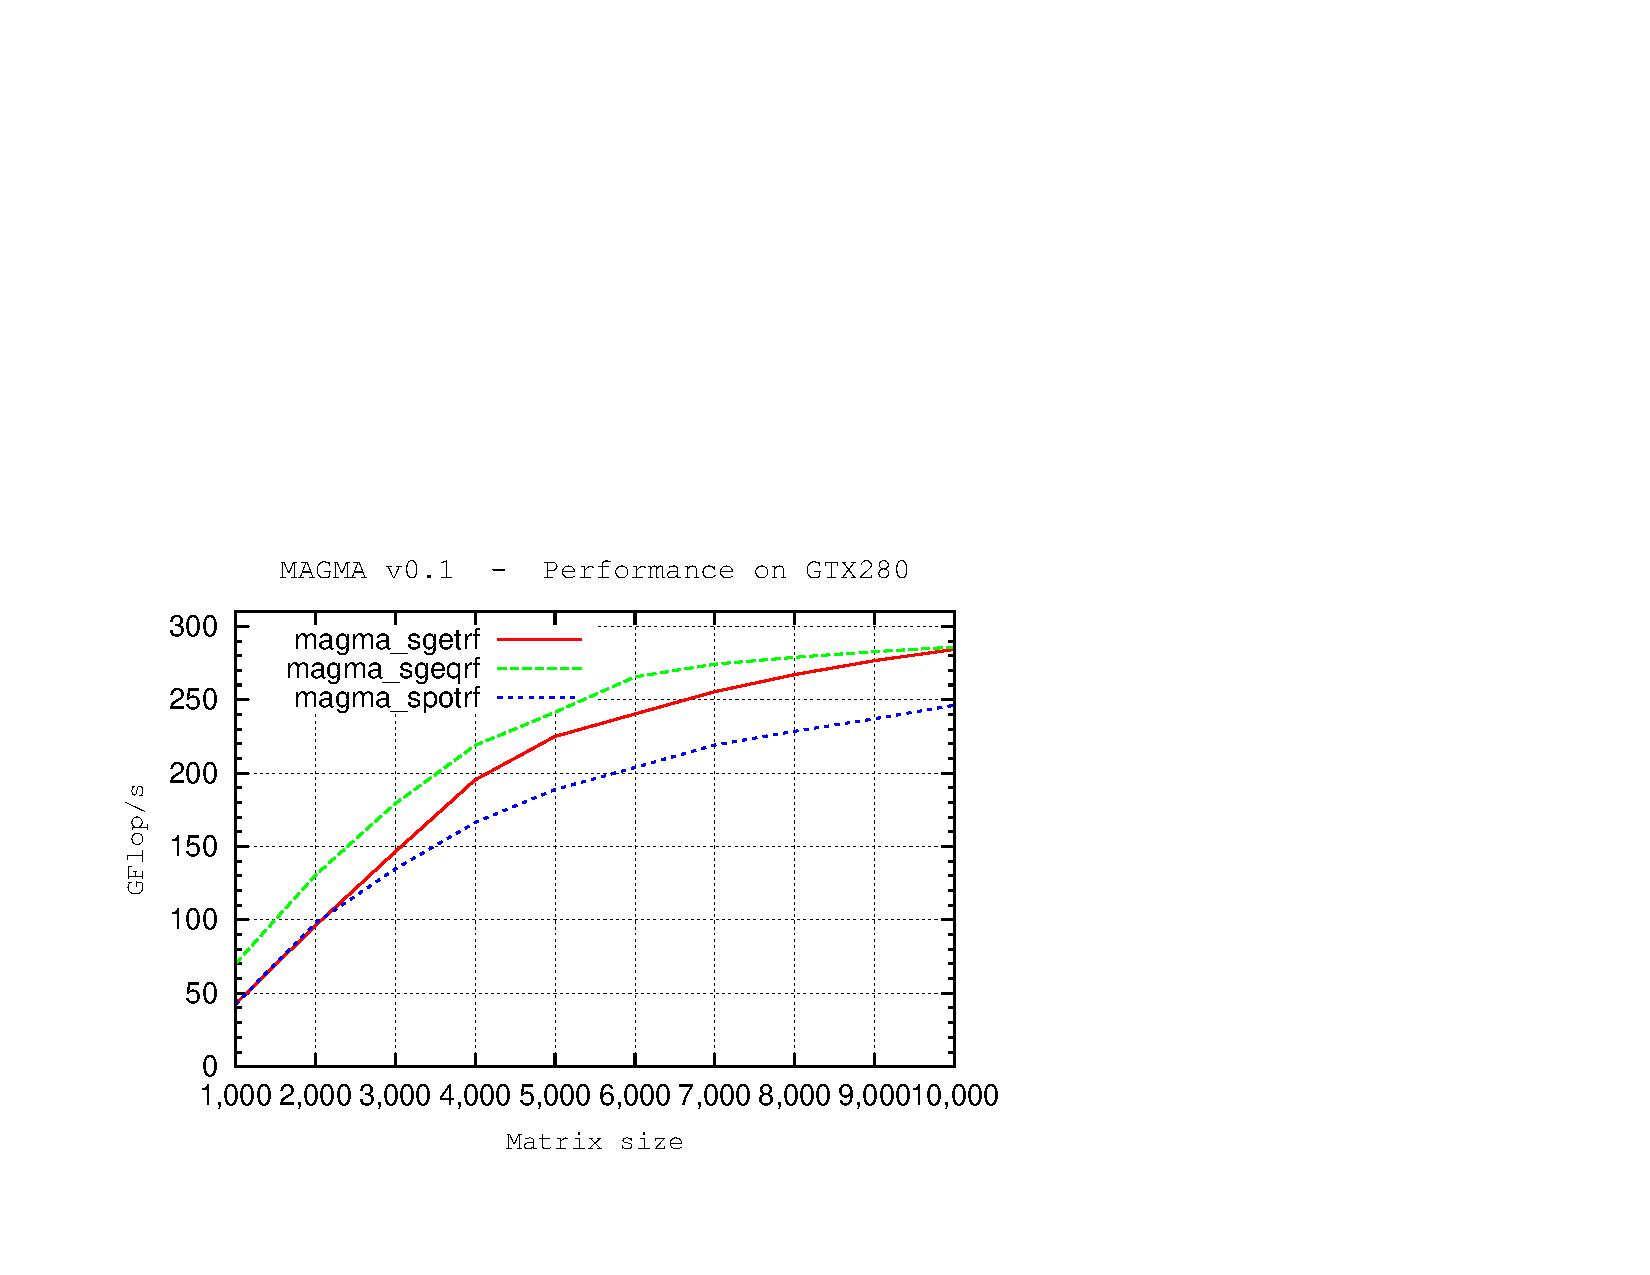
\includegraphics[width=7in]{sp-cpu.pdf}
          \caption{Performance of the {\bf CPU interface} 
                   one-sided factorizations.}
       \label{sp-cpu-performance}
       \end{figure}

       \begin{figure}[!ht]
          \centering
          \hspace{-5mm}
          \includegraphics[angle=-90,scale=0.7]{sp-gpu-v0.2.ps}
          %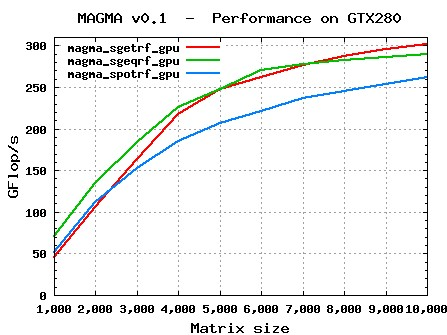
\includegraphics[width=5in]{sp-gpu.jpg}
          \caption{Performance of the {\bf GPU interface}
                   one-sided factorizations.}
       \label{sp-gpu-performance}
       \end{figure}
\newpage
%%%%%%%%%%%%%%%%%%%%%%%%%%%%%%%%%%%%%%%%%%%%%%%%%%%%%%%%%%%%%%%%%%%%%%%%%%%%%%%
\section{Double precision one-sided factorizations}
%%%%%%%%%%%%%%%%%%%%%%%%%%%%%%%%%%%%%%%%%%%%%%%%%%%%%%%%%%%%%%%%%%%%%%%%%%%%%%%
       \begin{figure}[!ht]
          \centering
          \hspace{-5mm}
          \includegraphics[angle=-90,scale=0.7]{dp-cpu-v0.2.ps}
          %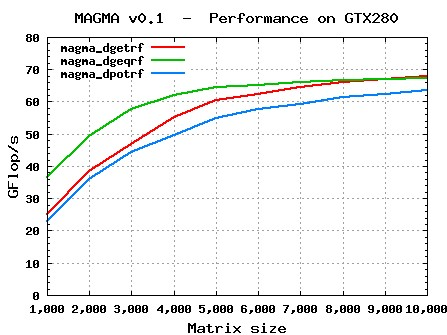
\includegraphics[width=5in]{dp-cpu.jpg}
          \caption{Performance of the {\bf CPU interface} 
                   one-sided factorizations.}
       \label{dp-cpu-performance}
       \end{figure}

       \begin{figure}[!ht]
          \centering
          \hspace{-5mm}
          \includegraphics[angle=-90,scale=0.7]{dp-gpu-v0.2.ps}
          %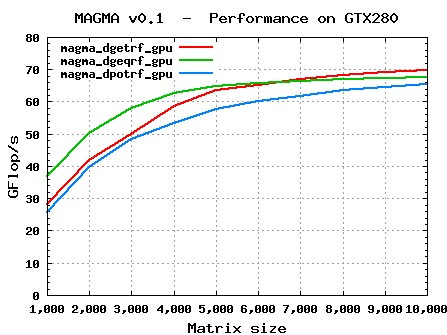
\includegraphics[width=5in]{dp-gpu.jpg}
          \caption{Performance of the {\bf GPU interface} 
                   one-sided factorizations.}
       \label{dp-gpu-performance}
       \end{figure}

\newpage
%%%%%%%%%%%%%%%%%%%%%%%%%%%%%%%%%%%%%%%%%%%%%%%%%%%%%%%%%%%%%%%%%%%%%%%%%%%%%%%
\section{Single complex one-sided factorizations}
%%%%%%%%%%%%%%%%%%%%%%%%%%%%%%%%%%%%%%%%%%%%%%%%%%%%%%%%%%%%%%%%%%%%%%%%%%%%%%%
       \begin{figure}[!ht]
          \centering
          \hspace{-5mm}
          \includegraphics[angle=-90,scale=0.7]{sc-cpu-v0.2.ps}
          %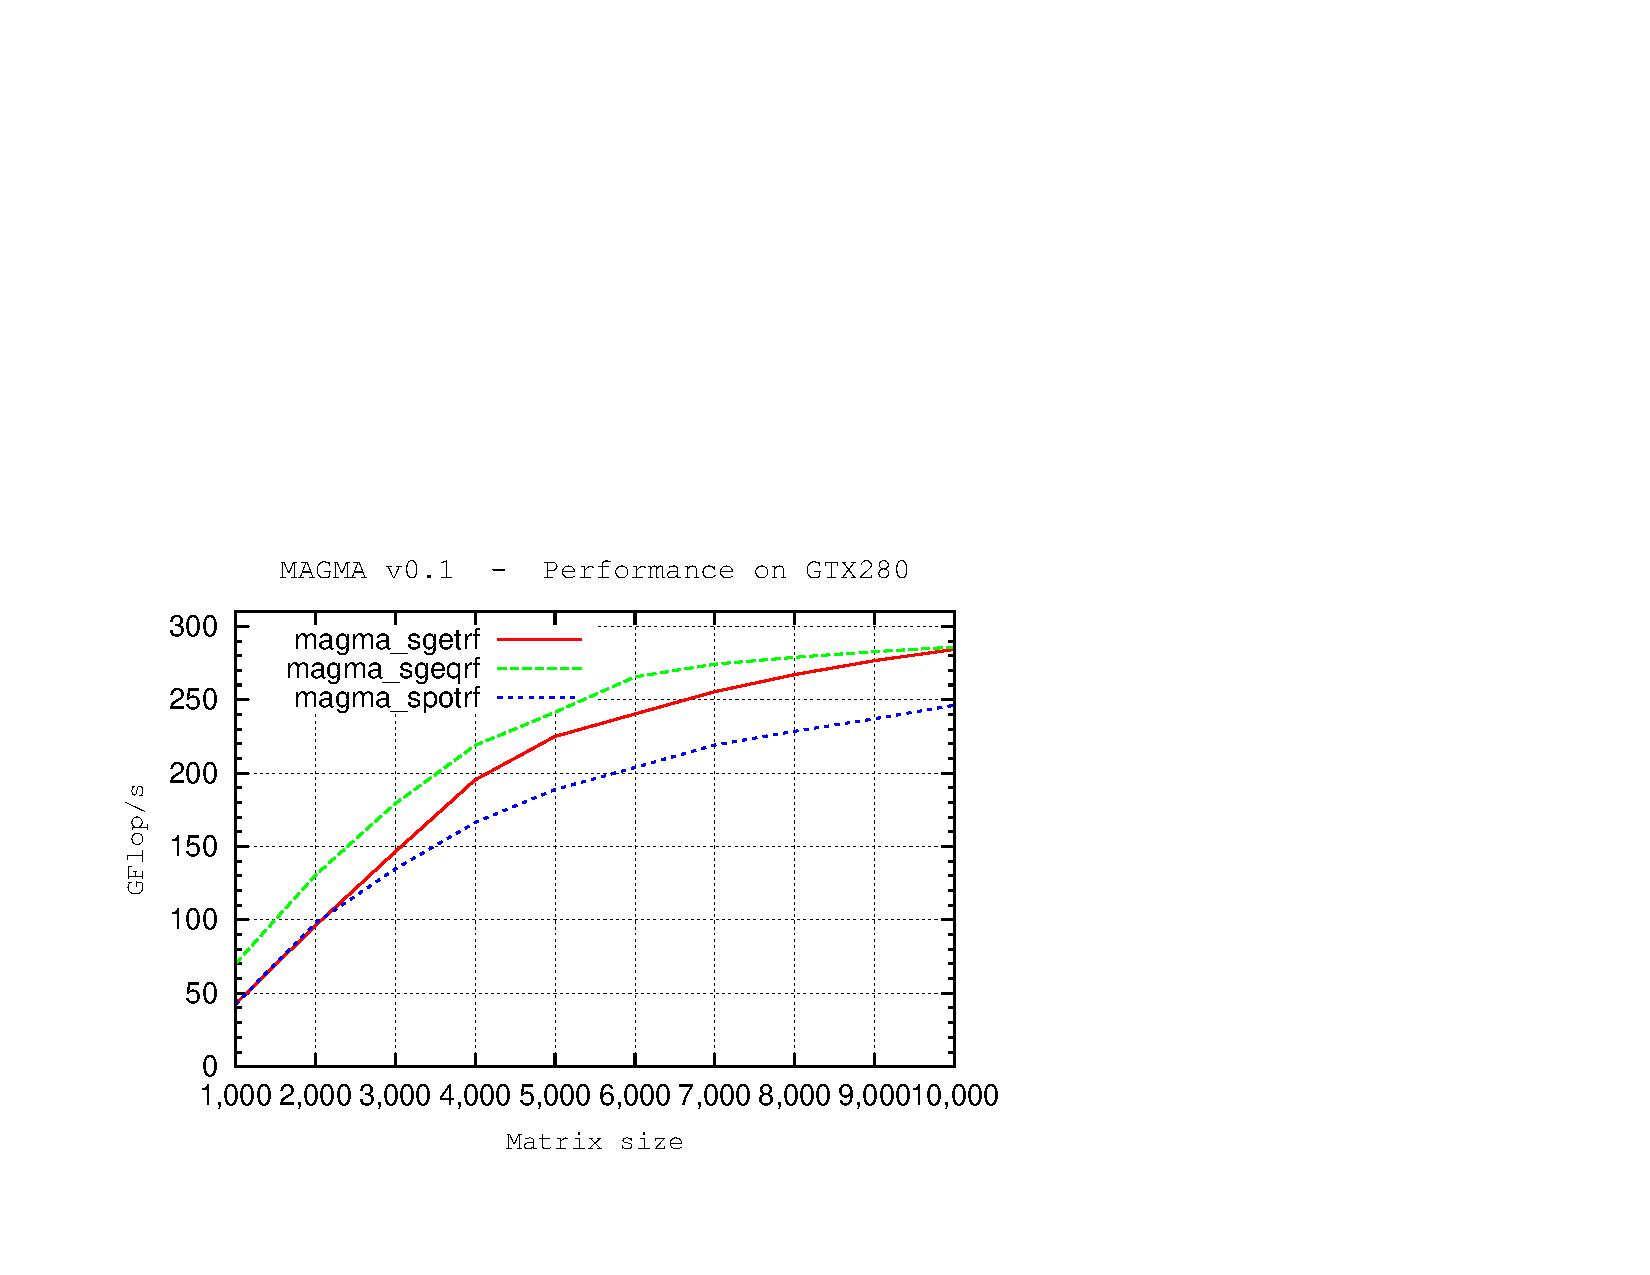
\includegraphics[width=7in]{sp-cpu.pdf}
          \caption{Performance of the {\bf CPU interface} 
                   one-sided factorizations.}
       \label{sp-cpu-performance}
       \end{figure}

       \begin{figure}[!ht]
          \centering
          \hspace{-5mm}
          \includegraphics[angle=-90,scale=0.7]{sc-gpu-v0.2.ps}
          %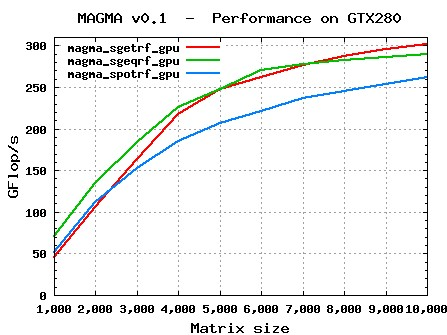
\includegraphics[width=5in]{sp-gpu.jpg}
          \caption{Performance of the {\bf GPU interface}
                   one-sided factorizations.}
       \label{sp-gpu-performance}
       \end{figure}

\newpage
%%%%%%%%%%%%%%%%%%%%%%%%%%%%%%%%%%%%%%%%%%%%%%%%%%%%%%%%%%%%%%%%%%%%%%%%%%%%%%%
\section{Double complex one-sided factorizations}
%%%%%%%%%%%%%%%%%%%%%%%%%%%%%%%%%%%%%%%%%%%%%%%%%%%%%%%%%%%%%%%%%%%%%%%%%%%%%%%
       \begin{figure}[!ht]
          \centering
          \hspace{-5mm}
          \includegraphics[angle=-90,scale=0.7]{dc-cpu-v0.2.ps}
          %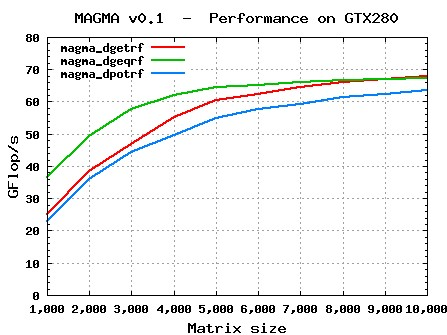
\includegraphics[width=5in]{dp-cpu.jpg}
          \caption{Performance of the {\bf CPU interface} 
                   one-sided factorizations.}
       \label{dp-cpu-performance}
       \end{figure}

       \begin{figure}[!ht]
          \centering
          \hspace{-5mm}
          \includegraphics[angle=-90,scale=0.7]{dc-gpu-v0.2.ps}
          %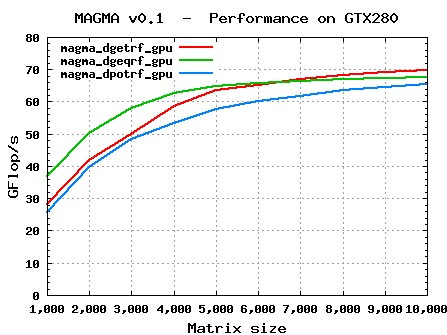
\includegraphics[width=5in]{dp-gpu.jpg}
          \caption{Performance of the {\bf GPU interface} 
                   one-sided factorizations.}
       \label{dp-gpu-performance}
       \end{figure}

\newpage
%%%%%%%%%%%%%%%%%%%%%%%%%%%%%%%%%%%%%%%%%%%%%%%%%%%%%%%%%%%%%%%%%%%%%%%%%%%%%%%
\section{LU-based linear solvers}
%%%%%%%%%%%%%%%%%%%%%%%%%%%%%%%%%%%%%%%%%%%%%%%%%%%%%%%%%%%%%%%%%%%%%%%%%%%%%%%
       \begin{figure}[!ht]
          \centering
          \hspace{-5mm}
          \includegraphics[angle=-90,scale=0.7]{lu-solve-v0.2.ps}
          %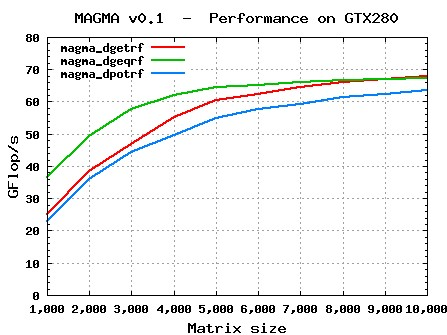
\includegraphics[width=5in]{dp-cpu.jpg}
          \caption{Performance of LU-based linear solvers.}
       \label{lu-solvers}
       \end{figure}

\newpage
%%%%%%%%%%%%%%%%%%%%%%%%%%%%%%%%%%%%%%%%%%%%%%%%%%%%%%%%%%%%%%%%%%%%%%%%%%%%%%%
\section{QR-based least squares solvers}
%%%%%%%%%%%%%%%%%%%%%%%%%%%%%%%%%%%%%%%%%%%%%%%%%%%%%%%%%%%%%%%%%%%%%%%%%%%%%%%
       \begin{figure}[!ht]
          \centering
          \hspace{-5mm}
          \includegraphics[angle=-90,scale=0.7]{qr-solve-v0.2.ps}
          %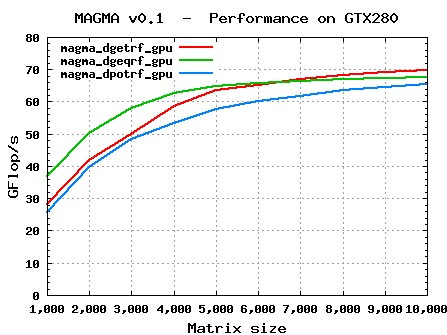
\includegraphics[width=5in]{dp-gpu.jpg}
          \caption{Performance of QR-based least squares solvers.}
       \label{qr-solvers}
       \end{figure}

\newpage
%%%%%%%%%%%%%%%%%%%%%%%%%%%%%%%%%%%%%%%%%%%%%%%%%%%%%%%%%%%%%%%%%%%%%%%%%%%%%%%
\section{Cholesky-based linear solvers}
%%%%%%%%%%%%%%%%%%%%%%%%%%%%%%%%%%%%%%%%%%%%%%%%%%%%%%%%%%%%%%%%%%%%%%%%%%%%%%%
       \begin{figure}[!ht]
          \centering
          \hspace{-5mm}
          \includegraphics[angle=-90,scale=0.7]{cholesky-solve-v0.2.ps}
          %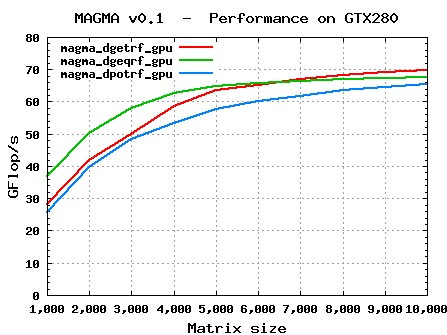
\includegraphics[width=5in]{dp-gpu.jpg}
          \caption{Performance of Cholesky-based linear solvers.}
       \label{cholesky-solvers}
       \end{figure}

%%%%%%%%%%%%%%%%%%%%%%%%%%%%%%%%%%%%%%%%%%%%%%%%%%%%%%%%%%%%%%%%%%%%%%%%%%%%%%%
%\addcontentsline{toc}{chapter}{Contributors}
%\chapter*{Contributors}

%%%%%%%%%%%%%%%%%%%%%%%%%%%%%%%%%%%%%%%%%%%%%%%%%%%%%%%%%%%%%%%%%%%%%%%%%%%%%%%


%%%%%%%%%%%%%%%%%%%%%%%%%%%%%%%%%%%%%%%%%%%%%%%%%%%%%%%%%%%%%%%%%%%%%%%%%%%%%%%
%\ackname{
\addcontentsline{toc}{chapter}{Acknowledgments}
\chapter*{Acknowledgments}
%{\bf Acknowledgments}.
This work is supported by Microsoft, the U.S. National Science Foundation,
and the U.S. Department of Energy. We thank NVIDIA and NVIDIA's Professor 
Partnership Program for their hardware donations.

%%%%%%%%%%%%%%%%%%%%%%%%%%%%%%%%%%%%%%%%%%%%%%%%%%%%%%%%%%%%%%%%%%%%%%%%%%%%%%%

\addcontentsline{toc}{chapter}{Bibliography}
\bibliographystyle{amsplain}
\bibliography{biblio}

\end{document}

set fichier=algochol
xfig -specialtext -latexfont -startlatexFont default $fichier.fig
fig2dev -L pstex $fichier.fig > $fichier.ps ; fig2dev -L pstex_t -p $fichier.ps $fichier.fig > $fichier.tex

%%%%%%%%%%%%%%%%%%%%%%%%%%%%%%%%%%%%%%%%%%%%%%%%%%%%%%%%%%%%%%%%%%%%%%%%%%%%%%%

